\documentclass[aspectratio=43,10pt]{beamer}

% ---------------------------------------------------------------- look & feel
\usetheme{Frankfurt}
\usepackage[T1]{fontenc}
\usepackage{lmodern}
\usepackage{amsmath,amssymb}
\usepackage{booktabs}
\usepackage{array}
\usepackage{multirow}
\usepackage{tikz}
\usetikzlibrary{arrows.meta,positioning,fit,calc,backgrounds}

\definecolor{tudnavy}{HTML}{0F2B46}
\definecolor{cNat}{HTML}{2A78D6}
\definecolor{cFsqF}{HTML}{EB6834}
\definecolor{cFsqJ}{HTML}{1BAF7A}
\definecolor{cJep}{HTML}{EDA100}
\definecolor{cGray}{HTML}{8A8A8A}

\setbeamercolor{structure}{fg=tudnavy}
\setbeamercolor{frametitle}{bg=tudnavy,fg=white}
\setbeamercolor{title}{bg=tudnavy,fg=white}
\setbeamercolor{section in head/foot}{bg=white,fg=tudnavy}
\setbeamercolor{subsection in head/foot}{bg=white,fg=tudnavy}
\setbeamercolor{footline}{bg=tudnavy,fg=white}
\setbeamercolor{item}{fg=tudnavy}
\setbeamercolor{block title}{bg=tudnavy,fg=white}
\setbeamercolor{block body}{bg=tudnavy!6}
\setbeamerfont{frametitle}{size=\large}
\setbeamertemplate{navigation symbols}{}
\setbeamertemplate{itemize items}[circle]
\setbeamertemplate{section in toc}[ball]
\setbeamertemplate{caption}[numbered]
\setbeamertemplate{frametitle}{%
  \nointerlineskip
  \begin{beamercolorbox}[wd=\paperwidth,ht=2.4ex,dp=1.1ex,leftskip=0.6em]{frametitle}
    \usebeamerfont{frametitle}\insertframetitle
  \end{beamercolorbox}}

% two-line footline as in the reference deck
\setbeamertemplate{footline}{%
  \leavevmode%
  \hbox{\begin{beamercolorbox}[wd=\paperwidth,ht=2.4ex,dp=0.9ex]{footline}%
    \scriptsize\hspace*{0.7em}\insertshortauthor\hfill\insertshortinstitute\hspace*{0.7em}%
  \end{beamercolorbox}}%
  \vskip0pt%
  \hbox{\begin{beamercolorbox}[wd=\paperwidth,ht=2.4ex,dp=1.1ex]{footline}%
    \scriptsize\hspace*{0.7em}\insertshorttitle\hfill\insertframenumber{} / \inserttotalframenumber\hspace*{0.7em}%
  \end{beamercolorbox}}}

\makeatletter\newcommand{\tabinput}[1]{\@@input #1 }\makeatother
% statistic tile for the ``Amount of Work'' slide
\newcommand{\stat}[3]{\node[tile] at (#1) {{\LARGE\bfseries\color{tudnavy}#2\par}\vspace{3pt}{\scriptsize #3\par}};}

% ---------------------------------------------------------------- title
\title[Universal Feature Extractor for Atari]{TOWARDS A UNIVERSAL FEATURE\\EXTRACTOR FOR ATARI GAMES}
\subtitle{Reconstruction, FSQ and Joint-Embedding Prediction}
\author{Sajid Ali Sadruddin}
\institute[Technische Universit\"at Dresden (TUD)]{Technische Universit\"at Dresden (TUD)}
\date{September 2026}
\titlegraphic{
\includegraphics[width=3.2cm]{figures/tud_logo.png}}

\begin{document}

\begin{frame}
  \titlepage
\end{frame}

\begin{frame}{Outline}
  \vfill
  \tableofcontents
  \vfill
\end{frame}

% =================================================================
\section{Introduction}

\begin{frame}{Motivation and Research Questions}
  \begin{itemize}\small\setlength\itemsep{0.2em}
    \item Every Atari game gives the agent the same input: 4 stacked $84\times84$ grey-scale frames
    \item Still, each agent trains its own CNN (NatureCNN) from scratch, using only the reward
    \item Many games look alike: sprites, balls, walls and scrolling backgrounds
    \item \textbf{Idea:} pre-train \textbf{one} encoder on many games and reuse it for PPO on
          every game
    \item Two design choices: the \textbf{objective} (reconstruct the pixels or predict the next
          latent) and the \textbf{usage} (frozen or fine-tuned)
  \end{itemize}
  \vspace{0.1em}
  \begin{block}{Research questions}
    \small
    \textbf{RQ1} Which objective gives the most useful features for PPO?\\
    \textbf{RQ2} Is it better to freeze or to fine-tune the encoder?\\
    \textbf{RQ3} Do the features work on games not seen in pre-training?\\
    \textbf{RQ4} What is the cost in GPU-hours and energy (kWh), and can the features be\\
    \phantom{\textbf{RQ4}} inspected, e.g.\ decoded back into images?
  \end{block}
\end{frame}

% =================================================================
\section{Related Work}

\begin{frame}{Related Work: Same Problem, One Model for Many Games}
  \centering
  {\footnotesize\setlength{\tabcolsep}{4pt}\renewcommand{\arraystretch}{1.1}
  \begin{tabular}{@{}>{\raggedright\arraybackslash}p{3.1cm}>{\raggedright\arraybackslash}p{3.6cm}>{\raggedright\arraybackslash}p{3.5cm}@{}}
    \toprule
    Approach & What they do & This work \\
    \midrule
    \textbf{One agent, many games}\newline{\scriptsize PopArt, Multi-Game DT, Scaled QL}
      & one network plays 40--57 games, trained with rewards
      & only the encoder is shared, no rewards \\\addlinespace[3pt]
    \textbf{Learning from experts}\newline{\scriptsize Policy Distillation, Actor-Mimic}
      & one network copies the experts of several games
      & experts only provide the data \\\addlinespace[3pt]
    \textbf{Transfer to a new game}\newline{\scriptsize Progressive Nets, Farebrother et al.}
      & reuse the features of one game for the next
      & one encoder from 11 games at once \\
    \bottomrule
  \end{tabular}}
\end{frame}

\begin{frame}{Related Work: From Images and Videos to Games}
  \centering
  {\footnotesize\setlength{\tabcolsep}{4pt}\renewcommand{\arraystretch}{1.1}
  \begin{tabular}{@{}>{\raggedright\arraybackslash}p{2.8cm}>{\raggedright\arraybackslash}p{3.6cm}>{\raggedright\arraybackslash}p{3.8cm}@{}}
    \toprule
    Method & Built for & Changed in this work \\
    \midrule
    \textbf{VAE, VQ-VAE, FSQ}
      & generating images, video and audio
      & encoder reused as the feature extractor for PPO; loss on moving pixels \\\addlinespace[3pt]
    \textbf{I-JEPA, V-JEPA}
      & images and videos: predict masked regions
      & predict the \emph{next} frame stack, given the action and the game; one model for 11 games \\\addlinespace[3pt]
    \textbf{TD-MPC2}
      & one world model for 80 robot-control tasks, used to plan
      & task embedding and SimNorm reused; no planning \\
    \bottomrule
  \end{tabular}}\\[0.6em]
  {\small Key difference: in games, the agent's \textbf{actions} change what happens next\par}
\end{frame}

\begin{frame}{Related Work: Model-Based vs.\ Model-Free RL}
  \centering
  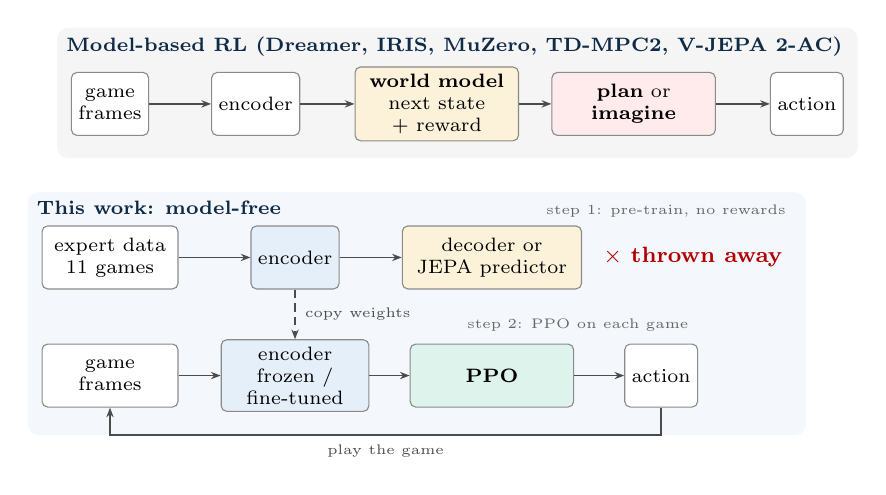
\begin{tikzpicture}[
    font=\scriptsize,
    box/.style={draw=cGray, rounded corners=2pt, align=center, inner sep=2.5pt, fill=white,
                minimum height=0.8cm},
    arr/.style={-{Stealth[length=3.5pt]}, draw=black!70, line width=0.6pt},
    lane/.style={rounded corners=4pt, inner sep=5pt},
    ttl/.style={font=\scriptsize\bfseries, anchor=north west, text=tudnavy}]

    % ---- model-based
    \node[box] (o1) at (0,0) {game\\frames};
    \node[box] (e1) at (1.85,0) {encoder};
    \node[box, fill=cJep!15, text width=1.9cm] (w1) at (4.15,0) {\textbf{world model}\\next state + reward};
    \node[box, fill=red!8, text width=1.9cm] (p1) at (6.65,0) {\textbf{plan} or\\\textbf{imagine}};
    \node[box] (a1) at (8.85,0) {action};
    \draw[arr] (o1) -- (e1); \draw[arr] (e1) -- (w1); \draw[arr] (w1) -- (p1); \draw[arr] (p1) -- (a1);
    \begin{scope}[on background layer]
      \node[lane, fill=gray!8, fit=(o1)(a1)(w1), inner ysep=10pt, yshift=4pt] (L1) {};
    \end{scope}
    \node[ttl] at (L1.north west) {Model-based RL (Dreamer, IRIS, MuZero, TD-MPC2, V-JEPA~2-AC)};

    % ---- this work, step 1
    \node[box, text width=1.55cm] (d2) at (0,-1.95) {expert data\\11 games};
    \node[box, fill=cNat!12] (e2) at (2.35,-1.95) {encoder};
    \node[box, fill=cJep!15, text width=2.1cm] (w2) at (4.85,-1.95) {decoder or\\JEPA predictor};
    \draw[arr] (d2) -- (e2); \draw[arr] (e2) -- (w2);
    \node[text=red!70!black, font=\footnotesize\bfseries, right=0.15cm of w2] (x2) {$\times$ thrown away};
    % ---- this work, step 2
    \node[box, text width=1.55cm] (o3) at (0,-3.45) {game\\frames};
    \node[box, fill=cNat!12, text width=1.7cm] (e3) at (2.35,-3.45) {encoder\\frozen / fine-tuned};
    \node[box, fill=cFsqJ!15, text width=1.9cm] (p3) at (4.85,-3.45) {\textbf{PPO}};
    \node[box] (a3) at (7.0,-3.45) {action};
    \draw[arr] (o3) -- (e3); \draw[arr] (e3) -- (p3); \draw[arr] (p3) -- (a3);
    \draw[arr, densely dashed] (e2) -- node[right, font=\tiny, text=black!70]{copy weights} (e3);
    \draw[arr] (a3.south) -- ++(0,-0.35) -| node[pos=0.25, below, font=\tiny, text=black!70]{play the game} (o3.south);
    \begin{scope}[on background layer]
      \node[lane, fill=cNat!5, fit=(d2)(o3)(x2)(a3), inner ysep=11pt, yshift=1pt] (L2) {};
    \end{scope}
    \node[ttl] at (L2.north west) {This work: model-free};
    \node[font=\tiny, text=black!60, anchor=east] at ([xshift=-4pt,yshift=-7pt]L2.north east) {step 1: pre-train, no rewards};
    \node[font=\tiny, text=black!60, anchor=south east] at ([yshift=1pt]a3.north east) {step 2: PPO on each game};
  \end{tikzpicture}
  \vspace{0.3em}
  \begin{itemize}\footnotesize\setlength\itemsep{0.15em}
    \item \textbf{Model-based:} the world model is used to choose the actions
    \item \textbf{This work:} the world model only trains the encoder; PPO chooses the actions
  \end{itemize}
\end{frame}

% =================================================================
\section{Methodology}

\begin{frame}{Data Collection}
  \centering
  \resizebox{\textwidth}{!}{% Data collection and training-time processing, used as % Data collection and training-time processing, used as % Data collection and training-time processing, used as \input{figures/data_pipeline}
\resizebox{\textwidth}{!}{%
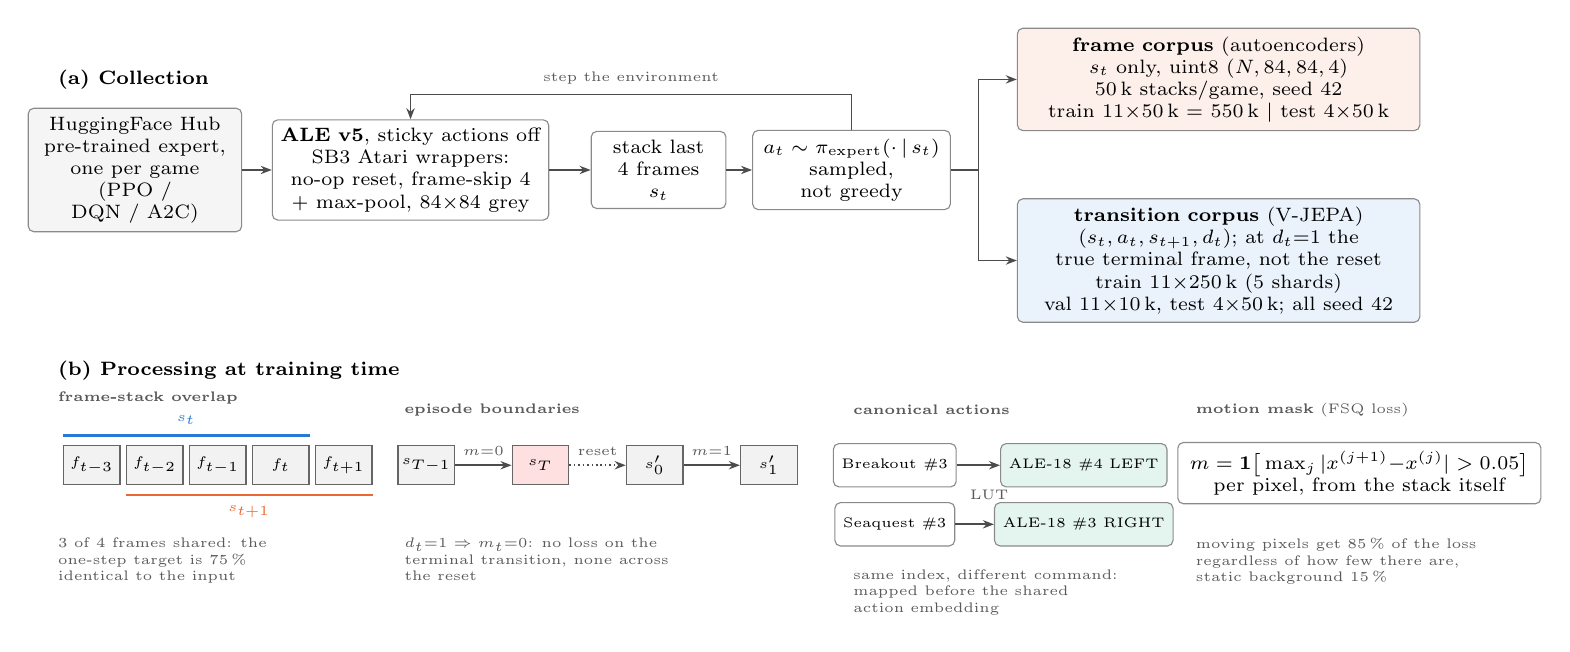
\begin{tikzpicture}[
  font=\scriptsize,
  box/.style={draw=cGray, rounded corners=2pt, align=center, inner sep=3pt, fill=white, minimum height=0.9cm},
  arr/.style={-{Stealth[length=4pt]}, draw=black!70, line width=0.6pt},
  fr/.style={draw=black!60, minimum width=0.72cm, minimum height=0.5cm, inner sep=0pt, font=\tiny},
  lab/.style={font=\tiny, text=black!65},
  ttl/.style={font=\scriptsize\bfseries, anchor=west}]

  % =========================================================== (a) collection
  \node[ttl] at (-1.1,3.35) {(a) Collection};
  \node[box, fill=gray!8, text width=2.5cm] (hub) at (0,2.2)
    {HuggingFace Hub\\pre-trained expert,\\one per game\\(PPO / DQN / A2C)};
  \node[box, text width=3.3cm] (env) at (3.5,2.2)
    {\textbf{ALE v5}, sticky actions off\\SB3 Atari wrappers: no-op reset, frame-skip 4 + max-pool, $84{\times}84$ grey};
  \node[box, text width=1.5cm] (stk) at (6.65,2.2) {stack last\\4 frames\\$s_t$};
  \node[box, text width=2.3cm] (pol) at (9.1,2.2) {$a_t\sim\pi_{\text{expert}}(\cdot\,|\,s_t)$\\sampled, not greedy};
  \draw[arr] (hub) -- (env); \draw[arr] (env) -- (stk); \draw[arr] (stk) -- (pol);
  \draw[arr] (pol.north) -- ++(0,0.45) -| node[pos=0.25, above, lab]{step the environment} (env.north);

  \node[box, fill=cFsqF!10, text width=4.9cm, anchor=west] (c1) at (11.2,3.35)
    {\textbf{frame corpus} (autoencoders)\\$s_t$ only, uint8 $(N,84,84,4)$\\50\,k stacks/game, seed 42\\train 11${\times}$50\,k = 550\,k $\mid$ test 4${\times}$50\,k};
  \node[box, fill=cNat!10, text width=4.9cm, anchor=west] (c2) at (11.2,1.05)
    {\textbf{transition corpus} (V-JEPA)\\$(s_t,a_t,s_{t+1},d_t)$; at $d_t{=}1$ the\\true terminal frame, not the reset\\train 11${\times}$250\,k (5 shards)\\val 11${\times}$10\,k, test 4${\times}$50\,k; all seed 42};
  \draw[arr] (pol.east) -- ++(0.35,0) |- (c1.west);
  \draw[arr] (pol.east) -- ++(0.35,0) |- (c2.west);

  % =========================================================== (b) processing
  \node[ttl] at (-1.1,-0.35) {(b) Processing at training time};

  % --- b1 frame overlap
  \node[lab, anchor=west] at (-1.1,-0.7) {\textbf{frame-stack overlap}};
  \foreach \i/\t in {0/$f_{t-3}$,1/$f_{t-2}$,2/$f_{t-1}$,3/$f_{t}$,4/$f_{t+1}$}
    {\node[fr, fill=gray!10] (f\i) at (-0.55+\i*0.8,-1.55) {\t};}
  \draw[cNat, line width=1pt] ([yshift=0.12cm]f0.north west) -- ([yshift=0.12cm]f3.north east)
     node[midway, above, font=\tiny, text=cNat] {$s_t$};
  \draw[cFsqF, line width=1pt] ([yshift=-0.12cm]f1.south west) -- ([yshift=-0.12cm]f4.south east)
     node[midway, below, font=\tiny, text=cFsqF] {$s_{t+1}$};
  \node[lab, align=left, anchor=north west] at (-1.1,-2.35) {3 of 4 frames shared: the\\one-step target is 75\,\%\\identical to the input};

  % --- b2 terminal mask
  \node[lab, anchor=west] at (3.3,-0.85) {\textbf{episode boundaries}};
  \node[fr, fill=gray!10] (e1) at (3.7,-1.55) {$s_{T-1}$};
  \node[fr, fill=red!12] (e2) at (5.15,-1.55) {$s_T$};
  \node[fr, fill=gray!10] (e3) at (6.6,-1.55) {$s'_0$};
  \node[fr, fill=gray!10] (e4) at (8.05,-1.55) {$s'_1$};
  \draw[arr] (e1) -- node[above, lab]{$m{=}0$} (e2);
  \draw[arr, densely dotted] (e2) -- node[above, lab]{reset} (e3);
  \draw[arr] (e3) -- node[above, lab]{$m{=}1$} (e4);
  \node[lab, align=left, anchor=north west] at (3.3,-2.35) {$d_t{=}1\Rightarrow m_t{=}0$: no loss on the\\terminal transition, none across\\the reset};

  % --- b3 action canonicalisation
  \node[lab, anchor=west] at (9.0,-0.85) {\textbf{canonical actions}};
  \node[box, minimum height=0.55cm, font=\tiny] (bk) at (9.65,-1.55) {Breakout \#3};
  \node[box, minimum height=0.55cm, font=\tiny] (sq) at (9.65,-2.3) {Seaquest \#3};
  \node[box, minimum height=0.55cm, font=\tiny, fill=cFsqJ!12] (l4) at (12.05,-1.55) {ALE-18 \#4 LEFT};
  \node[box, minimum height=0.55cm, font=\tiny, fill=cFsqJ!12] (r3) at (12.05,-2.3) {ALE-18 \#3 RIGHT};
  \draw[arr] (bk) -- (l4); \node[lab] at (10.85,-1.93) {LUT}; \draw[arr] (sq) -- (r3);
  \node[lab, align=left, anchor=north west] at (9.0,-2.75) {same index, different command:\\mapped before the shared\\action embedding};

  % --- b4 motion mask
  \node[lab, anchor=west] at (13.35,-0.85) {\textbf{motion mask} (FSQ loss)};
  \node[box, minimum height=0.55cm, text width=4.4cm, font=\scriptsize] (mm) at (15.55,-1.65)
    {\mbox{$m=\mathbf{1}\big[\max_j|x^{(j+1)}{-}x^{(j)}|>0.05\big]$}\\per pixel, from the stack itself};
  \node[lab, align=left, anchor=north west] at (13.35,-2.35) {moving pixels get 85\,\% of the loss\\regardless of how few there are,\\static background 15\,\%};
\end{tikzpicture}}

\resizebox{\textwidth}{!}{%
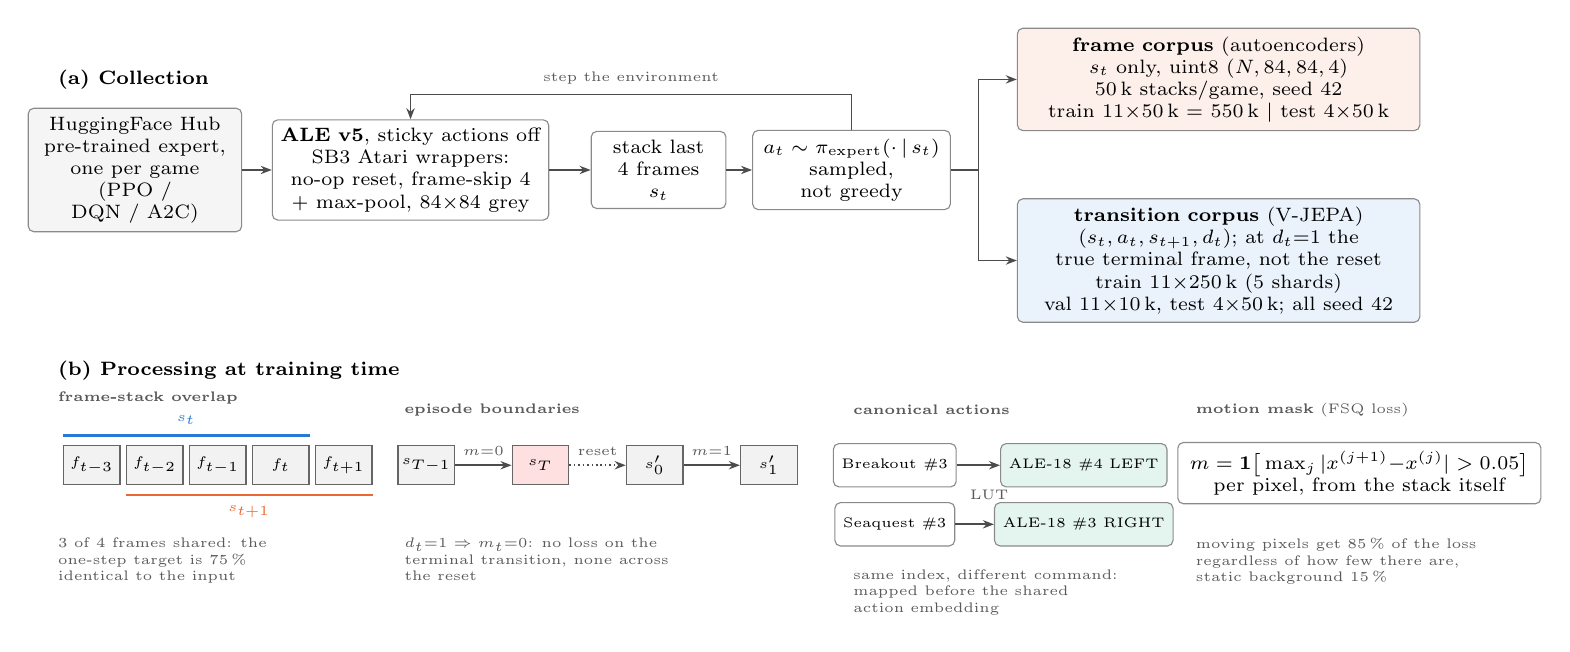
\begin{tikzpicture}[
  font=\scriptsize,
  box/.style={draw=cGray, rounded corners=2pt, align=center, inner sep=3pt, fill=white, minimum height=0.9cm},
  arr/.style={-{Stealth[length=4pt]}, draw=black!70, line width=0.6pt},
  fr/.style={draw=black!60, minimum width=0.72cm, minimum height=0.5cm, inner sep=0pt, font=\tiny},
  lab/.style={font=\tiny, text=black!65},
  ttl/.style={font=\scriptsize\bfseries, anchor=west}]

  % =========================================================== (a) collection
  \node[ttl] at (-1.1,3.35) {(a) Collection};
  \node[box, fill=gray!8, text width=2.5cm] (hub) at (0,2.2)
    {HuggingFace Hub\\pre-trained expert,\\one per game\\(PPO / DQN / A2C)};
  \node[box, text width=3.3cm] (env) at (3.5,2.2)
    {\textbf{ALE v5}, sticky actions off\\SB3 Atari wrappers: no-op reset, frame-skip 4 + max-pool, $84{\times}84$ grey};
  \node[box, text width=1.5cm] (stk) at (6.65,2.2) {stack last\\4 frames\\$s_t$};
  \node[box, text width=2.3cm] (pol) at (9.1,2.2) {$a_t\sim\pi_{\text{expert}}(\cdot\,|\,s_t)$\\sampled, not greedy};
  \draw[arr] (hub) -- (env); \draw[arr] (env) -- (stk); \draw[arr] (stk) -- (pol);
  \draw[arr] (pol.north) -- ++(0,0.45) -| node[pos=0.25, above, lab]{step the environment} (env.north);

  \node[box, fill=cFsqF!10, text width=4.9cm, anchor=west] (c1) at (11.2,3.35)
    {\textbf{frame corpus} (autoencoders)\\$s_t$ only, uint8 $(N,84,84,4)$\\50\,k stacks/game, seed 42\\train 11${\times}$50\,k = 550\,k $\mid$ test 4${\times}$50\,k};
  \node[box, fill=cNat!10, text width=4.9cm, anchor=west] (c2) at (11.2,1.05)
    {\textbf{transition corpus} (V-JEPA)\\$(s_t,a_t,s_{t+1},d_t)$; at $d_t{=}1$ the\\true terminal frame, not the reset\\train 11${\times}$250\,k (5 shards)\\val 11${\times}$10\,k, test 4${\times}$50\,k; all seed 42};
  \draw[arr] (pol.east) -- ++(0.35,0) |- (c1.west);
  \draw[arr] (pol.east) -- ++(0.35,0) |- (c2.west);

  % =========================================================== (b) processing
  \node[ttl] at (-1.1,-0.35) {(b) Processing at training time};

  % --- b1 frame overlap
  \node[lab, anchor=west] at (-1.1,-0.7) {\textbf{frame-stack overlap}};
  \foreach \i/\t in {0/$f_{t-3}$,1/$f_{t-2}$,2/$f_{t-1}$,3/$f_{t}$,4/$f_{t+1}$}
    {\node[fr, fill=gray!10] (f\i) at (-0.55+\i*0.8,-1.55) {\t};}
  \draw[cNat, line width=1pt] ([yshift=0.12cm]f0.north west) -- ([yshift=0.12cm]f3.north east)
     node[midway, above, font=\tiny, text=cNat] {$s_t$};
  \draw[cFsqF, line width=1pt] ([yshift=-0.12cm]f1.south west) -- ([yshift=-0.12cm]f4.south east)
     node[midway, below, font=\tiny, text=cFsqF] {$s_{t+1}$};
  \node[lab, align=left, anchor=north west] at (-1.1,-2.35) {3 of 4 frames shared: the\\one-step target is 75\,\%\\identical to the input};

  % --- b2 terminal mask
  \node[lab, anchor=west] at (3.3,-0.85) {\textbf{episode boundaries}};
  \node[fr, fill=gray!10] (e1) at (3.7,-1.55) {$s_{T-1}$};
  \node[fr, fill=red!12] (e2) at (5.15,-1.55) {$s_T$};
  \node[fr, fill=gray!10] (e3) at (6.6,-1.55) {$s'_0$};
  \node[fr, fill=gray!10] (e4) at (8.05,-1.55) {$s'_1$};
  \draw[arr] (e1) -- node[above, lab]{$m{=}0$} (e2);
  \draw[arr, densely dotted] (e2) -- node[above, lab]{reset} (e3);
  \draw[arr] (e3) -- node[above, lab]{$m{=}1$} (e4);
  \node[lab, align=left, anchor=north west] at (3.3,-2.35) {$d_t{=}1\Rightarrow m_t{=}0$: no loss on the\\terminal transition, none across\\the reset};

  % --- b3 action canonicalisation
  \node[lab, anchor=west] at (9.0,-0.85) {\textbf{canonical actions}};
  \node[box, minimum height=0.55cm, font=\tiny] (bk) at (9.65,-1.55) {Breakout \#3};
  \node[box, minimum height=0.55cm, font=\tiny] (sq) at (9.65,-2.3) {Seaquest \#3};
  \node[box, minimum height=0.55cm, font=\tiny, fill=cFsqJ!12] (l4) at (12.05,-1.55) {ALE-18 \#4 LEFT};
  \node[box, minimum height=0.55cm, font=\tiny, fill=cFsqJ!12] (r3) at (12.05,-2.3) {ALE-18 \#3 RIGHT};
  \draw[arr] (bk) -- (l4); \node[lab] at (10.85,-1.93) {LUT}; \draw[arr] (sq) -- (r3);
  \node[lab, align=left, anchor=north west] at (9.0,-2.75) {same index, different command:\\mapped before the shared\\action embedding};

  % --- b4 motion mask
  \node[lab, anchor=west] at (13.35,-0.85) {\textbf{motion mask} (FSQ loss)};
  \node[box, minimum height=0.55cm, text width=4.4cm, font=\scriptsize] (mm) at (15.55,-1.65)
    {\mbox{$m=\mathbf{1}\big[\max_j|x^{(j+1)}{-}x^{(j)}|>0.05\big]$}\\per pixel, from the stack itself};
  \node[lab, align=left, anchor=north west] at (13.35,-2.35) {moving pixels get 85\,\% of the loss\\regardless of how few there are,\\static background 15\,\%};
\end{tikzpicture}}

\resizebox{\textwidth}{!}{%
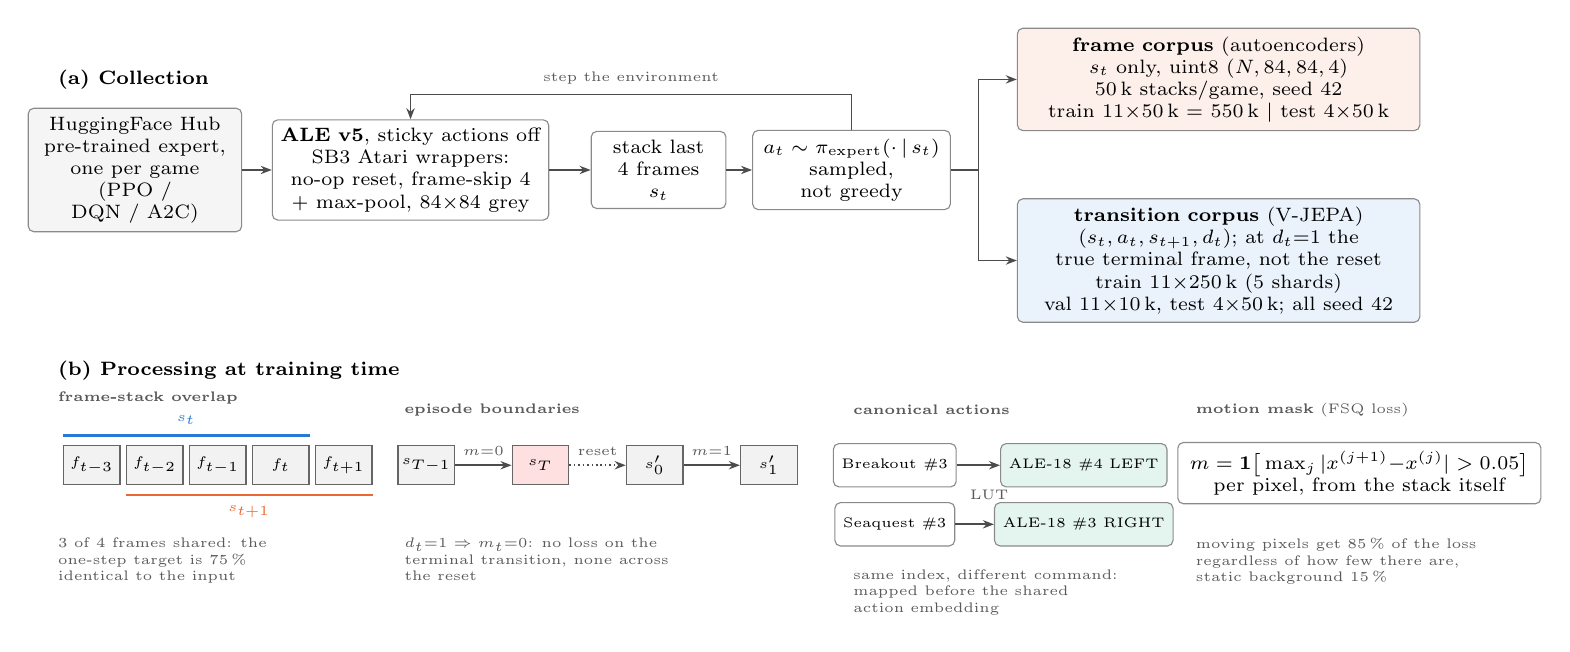
\begin{tikzpicture}[
  font=\scriptsize,
  box/.style={draw=cGray, rounded corners=2pt, align=center, inner sep=3pt, fill=white, minimum height=0.9cm},
  arr/.style={-{Stealth[length=4pt]}, draw=black!70, line width=0.6pt},
  fr/.style={draw=black!60, minimum width=0.72cm, minimum height=0.5cm, inner sep=0pt, font=\tiny},
  lab/.style={font=\tiny, text=black!65},
  ttl/.style={font=\scriptsize\bfseries, anchor=west}]

  % =========================================================== (a) collection
  \node[ttl] at (-1.1,3.35) {(a) Collection};
  \node[box, fill=gray!8, text width=2.5cm] (hub) at (0,2.2)
    {HuggingFace Hub\\pre-trained expert,\\one per game\\(PPO / DQN / A2C)};
  \node[box, text width=3.3cm] (env) at (3.5,2.2)
    {\textbf{ALE v5}, sticky actions off\\SB3 Atari wrappers: no-op reset, frame-skip 4 + max-pool, $84{\times}84$ grey};
  \node[box, text width=1.5cm] (stk) at (6.65,2.2) {stack last\\4 frames\\$s_t$};
  \node[box, text width=2.3cm] (pol) at (9.1,2.2) {$a_t\sim\pi_{\text{expert}}(\cdot\,|\,s_t)$\\sampled, not greedy};
  \draw[arr] (hub) -- (env); \draw[arr] (env) -- (stk); \draw[arr] (stk) -- (pol);
  \draw[arr] (pol.north) -- ++(0,0.45) -| node[pos=0.25, above, lab]{step the environment} (env.north);

  \node[box, fill=cFsqF!10, text width=4.9cm, anchor=west] (c1) at (11.2,3.35)
    {\textbf{frame corpus} (autoencoders)\\$s_t$ only, uint8 $(N,84,84,4)$\\50\,k stacks/game, seed 42\\train 11${\times}$50\,k = 550\,k $\mid$ test 4${\times}$50\,k};
  \node[box, fill=cNat!10, text width=4.9cm, anchor=west] (c2) at (11.2,1.05)
    {\textbf{transition corpus} (V-JEPA)\\$(s_t,a_t,s_{t+1},d_t)$; at $d_t{=}1$ the\\true terminal frame, not the reset\\train 11${\times}$250\,k (5 shards)\\val 11${\times}$10\,k, test 4${\times}$50\,k; all seed 42};
  \draw[arr] (pol.east) -- ++(0.35,0) |- (c1.west);
  \draw[arr] (pol.east) -- ++(0.35,0) |- (c2.west);

  % =========================================================== (b) processing
  \node[ttl] at (-1.1,-0.35) {(b) Processing at training time};

  % --- b1 frame overlap
  \node[lab, anchor=west] at (-1.1,-0.7) {\textbf{frame-stack overlap}};
  \foreach \i/\t in {0/$f_{t-3}$,1/$f_{t-2}$,2/$f_{t-1}$,3/$f_{t}$,4/$f_{t+1}$}
    {\node[fr, fill=gray!10] (f\i) at (-0.55+\i*0.8,-1.55) {\t};}
  \draw[cNat, line width=1pt] ([yshift=0.12cm]f0.north west) -- ([yshift=0.12cm]f3.north east)
     node[midway, above, font=\tiny, text=cNat] {$s_t$};
  \draw[cFsqF, line width=1pt] ([yshift=-0.12cm]f1.south west) -- ([yshift=-0.12cm]f4.south east)
     node[midway, below, font=\tiny, text=cFsqF] {$s_{t+1}$};
  \node[lab, align=left, anchor=north west] at (-1.1,-2.35) {3 of 4 frames shared: the\\one-step target is 75\,\%\\identical to the input};

  % --- b2 terminal mask
  \node[lab, anchor=west] at (3.3,-0.85) {\textbf{episode boundaries}};
  \node[fr, fill=gray!10] (e1) at (3.7,-1.55) {$s_{T-1}$};
  \node[fr, fill=red!12] (e2) at (5.15,-1.55) {$s_T$};
  \node[fr, fill=gray!10] (e3) at (6.6,-1.55) {$s'_0$};
  \node[fr, fill=gray!10] (e4) at (8.05,-1.55) {$s'_1$};
  \draw[arr] (e1) -- node[above, lab]{$m{=}0$} (e2);
  \draw[arr, densely dotted] (e2) -- node[above, lab]{reset} (e3);
  \draw[arr] (e3) -- node[above, lab]{$m{=}1$} (e4);
  \node[lab, align=left, anchor=north west] at (3.3,-2.35) {$d_t{=}1\Rightarrow m_t{=}0$: no loss on the\\terminal transition, none across\\the reset};

  % --- b3 action canonicalisation
  \node[lab, anchor=west] at (9.0,-0.85) {\textbf{canonical actions}};
  \node[box, minimum height=0.55cm, font=\tiny] (bk) at (9.65,-1.55) {Breakout \#3};
  \node[box, minimum height=0.55cm, font=\tiny] (sq) at (9.65,-2.3) {Seaquest \#3};
  \node[box, minimum height=0.55cm, font=\tiny, fill=cFsqJ!12] (l4) at (12.05,-1.55) {ALE-18 \#4 LEFT};
  \node[box, minimum height=0.55cm, font=\tiny, fill=cFsqJ!12] (r3) at (12.05,-2.3) {ALE-18 \#3 RIGHT};
  \draw[arr] (bk) -- (l4); \node[lab] at (10.85,-1.93) {LUT}; \draw[arr] (sq) -- (r3);
  \node[lab, align=left, anchor=north west] at (9.0,-2.75) {same index, different command:\\mapped before the shared\\action embedding};

  % --- b4 motion mask
  \node[lab, anchor=west] at (13.35,-0.85) {\textbf{motion mask} (FSQ loss)};
  \node[box, minimum height=0.55cm, text width=4.4cm, font=\scriptsize] (mm) at (15.55,-1.65)
    {\mbox{$m=\mathbf{1}\big[\max_j|x^{(j+1)}{-}x^{(j)}|>0.05\big]$}\\per pixel, from the stack itself};
  \node[lab, align=left, anchor=north west] at (13.35,-2.35) {moving pixels get 85\,\% of the loss\\regardless of how few there are,\\static background 15\,\%};
\end{tikzpicture}}
}
  \vspace{0.4em}
  \begin{itemize}\small\setlength\itemsep{0.3em}
    \item Random play rarely leaves the first screen, so expert agents from HuggingFace were used
    \item Actions were sampled from the expert policy, so some play is sub-optimal
    \item 11 games for pre-training, 4 games held out for testing
  \end{itemize}
\end{frame}

\begin{frame}{The Atari Games}
  \centering
  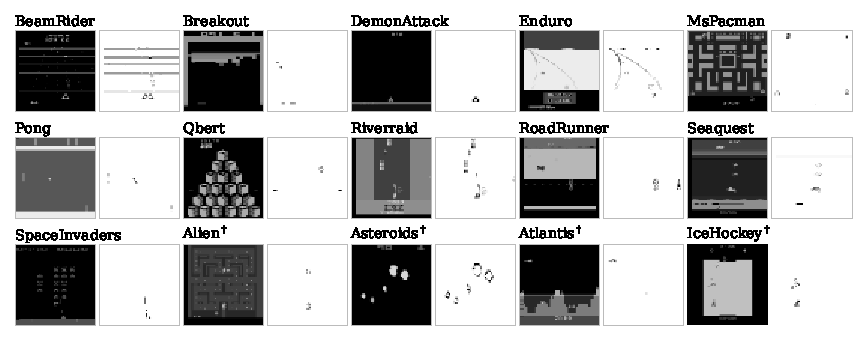
\includegraphics[width=0.92\textwidth]{figures/games_grid.pdf}\\[0.1em]
  {\scriptsize Frame $t$ (left) and the change to the next frame (right); $^\dagger$\,held-out games}
  \begin{itemize}\footnotesize\setlength\itemsep{0.1em}
    \item Same input shape, very different content: from 1\% to 95\% black pixels
    \item In most games less than 4\% of the pixels move: what matters are small sprites
    \item 4 to 18 actions, and the same action index means a different button in each game
  \end{itemize}
\end{frame}

\begin{frame}{Autoencoders}
  \centering
  \begin{tikzpicture}[font=\scriptsize,
     arr/.style={-{Stealth[length=3.5pt]}, draw=black!70, line width=0.6pt},
     pan/.style={draw=cGray, rounded corners=3pt, fill=gray!4, minimum width=3.0cm, minimum height=2.25cm},
     cell/.style={draw=black!50, minimum size=0.17cm, inner sep=0pt}]
    % ---- general principle
    \node[inner sep=1pt] (in) at (0,0) {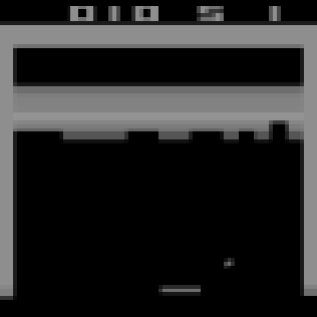
\includegraphics[width=1.55cm]{figures/ae_input_breakout.png}};
    \node[below=1pt of in, font=\tiny] {input frame};
    \filldraw[fill=cNat!20, draw=cNat] (1.15,-0.75) -- (2.85,-0.32) -- (2.85,0.32) -- (1.15,0.75) -- cycle;
    \node at (2.0,0) {\textbf{encoder}};
    \node[draw=cJep, fill=cJep!25, rounded corners=2pt, minimum width=1.35cm, minimum height=0.64cm] (z) at (3.75,0) {\textbf{bottleneck}};
    \filldraw[fill=cFsqJ!20, draw=cFsqJ] (4.65,-0.32) -- (6.35,-0.75) -- (6.35,0.75) -- (4.65,0.32) -- cycle;
    \node at (5.5,0) {\textbf{decoder}};
    \node[inner sep=1pt] (out) at (7.5,0) {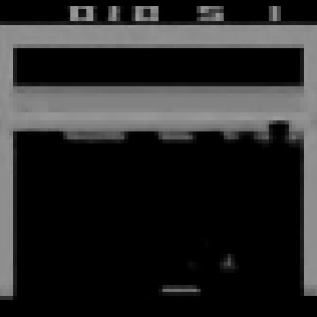
\includegraphics[width=1.55cm]{figures/ae_recon_fsq_breakout.png}};
    \node[below=1pt of out, font=\tiny] {reconstruction};
    \draw[arr] (in.east) -- (1.15,0); \draw[arr] (2.85,0) -- (z.west);
    \draw[arr] (z.east) -- (4.65,0); \draw[arr] (6.35,0) -- (out.west);
    \draw[{Stealth[length=3.5pt]}-{Stealth[length=3.5pt]}, densely dashed, red!60!black, line width=0.6pt]
      (in.north) -- ++(0,0.3) -| node[pos=0.25, above, text=red!60!black]{loss: difference between input and reconstruction} (out.north);
    \node[font=\tiny, text=black!60] at (3.75,-0.98) {after training, only the encoder is kept for PPO};

    % ---- three bottlenecks
    \node[pan] (p1) at (0.55,-2.75) {};
    \node[font=\scriptsize\bfseries, text=tudnavy] at ([yshift=-0.22cm]p1.north) {Standard VAE};
    \node[draw=cNat, fill=cNat!15, minimum width=0.4cm, minimum height=0.42cm, inner sep=0pt] (mu) at (-0.6,-2.6) {$\mu$};
    \node[draw=cNat, fill=cNat!15, minimum width=0.4cm, minimum height=0.42cm, inner sep=0pt] (sg) at (-0.12,-2.6) {$\sigma$};
    \node[anchor=west, inner sep=1pt] (zz) at (0.35,-2.6) {$z\sim\mathcal{N}(\mu,\sigma^2)$};
    \draw[arr] (sg) -- (zz);
    \node[text width=2.8cm, align=center, font=\tiny] at (0.55,-3.4) {one vector of 256 numbers\\(too coarse for small sprites)};

    \node[pan] (p2) at (3.75,-2.75) {};
    \node[font=\scriptsize\bfseries, text=tudnavy] at ([yshift=-0.22cm]p2.north) {Residual VQ-VAE};
    \foreach \i in {0,1,2} \foreach \j in {0,1,2}
      {\node[cell, fill=white] at (2.55+\i*0.17,-2.43-\j*0.17) {};}
    \node[cell, fill=cFsqF!70] (hc) at (2.72,-2.6) {};
    \foreach \k/\c in {0/cNat!50,1/cFsqJ!50,2/cFsqF!70,3/cJep!50,4/cGray!50}
      {\node[cell, fill=\c, minimum size=0.22cm] (cb\k) at (3.85+\k*0.26,-2.6) {};}
    \draw[cFsqF, line width=0.8pt] (cb2.south west) rectangle (cb2.north east);
    \draw[arr] (3.1,-2.6) -- (3.68,-2.6);
    \node[font=\tiny] at (4.37,-2.32) {codebook};
    \node[text width=2.8cm, align=center, font=\tiny] at (3.75,-3.4) {$21{\times}21$ grid; each cell is replaced\\by the nearest of 512 code vectors};

    \node[pan] (p3) at (6.95,-2.75) {};
    \node[font=\scriptsize\bfseries, text=tudnavy] at ([yshift=-0.22cm]p3.north) {FSQ-VAE};
    \draw[black!60] (6.15,-2.65) -- (7.75,-2.65);
    \foreach \t in {0,1,2,3,4} {\draw[black!60] (6.15+\t*0.4,-2.58) -- (6.15+\t*0.4,-2.72);}
    \fill[cFsqF] (6.73,-2.43) circle (1.6pt);
    \draw[arr, cFsqF] (6.73,-2.43) -- (6.57,-2.6);
    \node[font=\tiny] at (6.95,-2.9) {round to the nearest level};
    \node[text width=2.8cm, align=center, font=\tiny] at (6.95,-3.4) {4 channels with $L=[8,5,5,3]$\\levels; no codebook to learn};
  \end{tikzpicture}\\[0.4em]
  \begin{itemize}\footnotesize\setlength\itemsep{0.1em}
    \item Small moving objects got lost, so moving pixels get a higher weight in the loss
          (FSQ-VAE: 85\% of the loss)
  \end{itemize}
\end{frame}

\begin{frame}{V-JEPA World Model}
  \centering
  \resizebox{\textwidth}{!}{% V-JEPA v2 architecture (atari-DQN-v2/JEPA.py), used as % V-JEPA v2 architecture (atari-DQN-v2/JEPA.py), used as % V-JEPA v2 architecture (atari-DQN-v2/JEPA.py), used as \input{figures/jepa_arch}
\resizebox{\textwidth}{!}{%
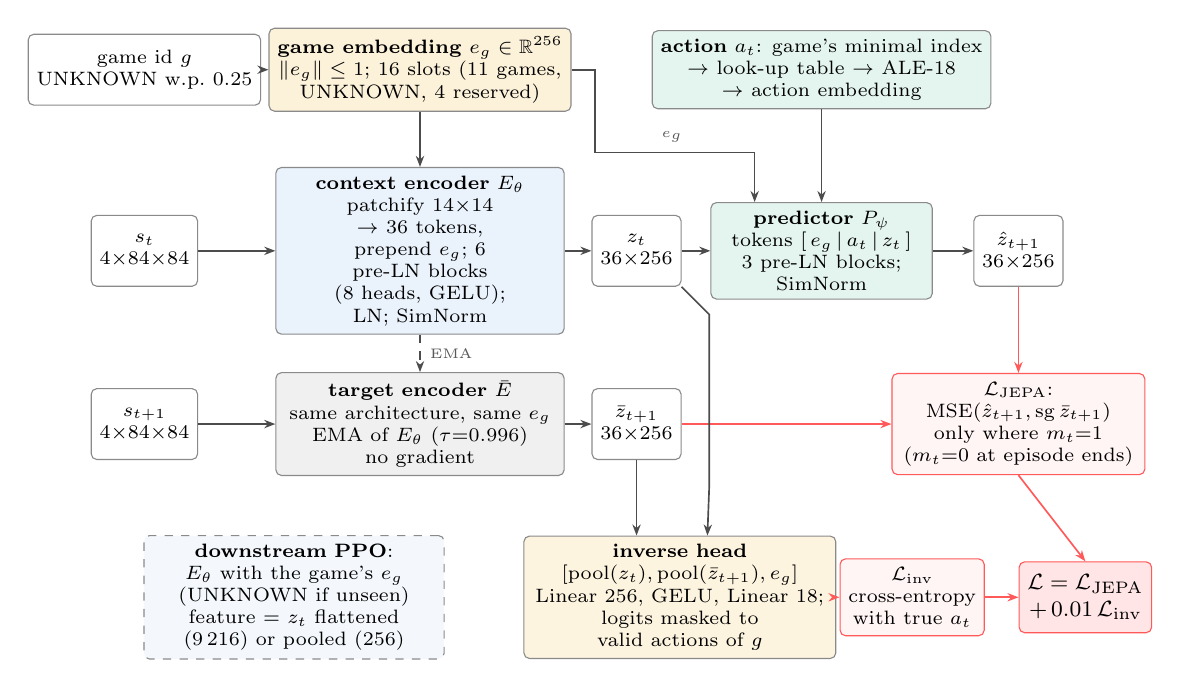
\begin{tikzpicture}[
  font=\scriptsize,
  box/.style={draw=cGray, rounded corners=2pt, align=center, inner sep=3pt, fill=white,
              minimum height=0.9cm},
  arr/.style={-{Stealth[length=4pt]}, draw=black!70, line width=0.6pt},
  larr/.style={-{Stealth[length=4pt]}, draw=red!65, line width=0.6pt},
  lab/.style={font=\tiny, text=black!65}]

  % ---------------------------------------------------------------- conditioning (top row)
  \node[box] (drop) at (0,4.5) {game id $g$\\UNKNOWN w.p.\ 0.25};
  \node[box, fill=cJep!15] (env) at (3.5,4.5)
    {\textbf{game embedding} $e_g\in\mathbb{R}^{256}$\\$\|e_g\|\le1$; 16 slots (11 games,\\UNKNOWN, 4 reserved)};
  \node[box, fill=cFsqJ!12] (act) at (8.6,4.5)
    {\textbf{action} $a_t$: game's minimal index\\$\to$ look-up table $\to$ ALE-18\\$\to$ action embedding};
  \draw[arr] (drop) -- (env);

  % ---------------------------------------------------------------- online branch
  \node[box] (st) at (0,2.2) {$s_t$\\$4{\times}84{\times}84$};
  \node[box, fill=cNat!10, text width=3.45cm] (ce) at (3.5,2.2)
    {\textbf{context encoder} $E_\theta$\\patchify $14{\times}14$ $\to$ 36 tokens,\\prepend $e_g$; 6 pre-LN blocks\\(8 heads, GELU); LN; SimNorm};
  \node[box] (zt) at (6.25,2.2) {$z_t$\\$36{\times}256$};
  \node[box, fill=cFsqJ!12, text width=2.6cm] (pr) at (8.6,2.2)
    {\textbf{predictor} $P_\psi$\\tokens $[\,e_g\,|\,a_t\,|\,z_t\,]$\\3 pre-LN blocks; SimNorm};
  \node[box] (zh) at (11.1,2.2) {$\hat z_{t+1}$\\$36{\times}256$};
  \draw[arr] (st) -- (ce); \draw[arr] (ce) -- (zt); \draw[arr] (zt) -- (pr); \draw[arr] (pr) -- (zh);
  \draw[arr] (env) -- (ce);
  \draw[arr] (act) -- (pr);
  \coordinate (ebend) at (7.75,3.45);
  \draw[arr] (env.east) -- ++(0.3,0) |- (ebend) -- (ebend |- pr.north);
  \node[lab, above] at (6.7,3.45) {$e_g$};

  % ---------------------------------------------------------------- target branch
  \node[box] (sn) at (0,0) {$s_{t+1}$\\$4{\times}84{\times}84$};
  \node[box, fill=gray!12, text width=3.45cm] (te) at (3.5,0)
    {\textbf{target encoder} $\bar E$\\same architecture, same $e_g$\\EMA of $E_\theta$ ($\tau{=}0.996$)\\no gradient};
  \node[box] (zb) at (6.25,0) {$\bar z_{t+1}$\\$36{\times}256$};
  \draw[arr] (sn) -- (te); \draw[arr] (te) -- (zb);
  \draw[arr, dashed] (ce) -- node[right, lab]{EMA} (te);

  % ---------------------------------------------------------------- losses
  \node[box, draw=red!65, fill=red!4, text width=3.0cm] (lj) at (11.1,0)
    {$\mathcal{L}_{\text{JEPA}}$: MSE$(\hat z_{t+1},\operatorname{sg}\bar z_{t+1})$\\only where $m_t{=}1$\\($m_t{=}0$ at episode ends)};
  \draw[larr] (zh) -- (lj);
  \draw[larr] (zb) -- (lj);

  \node[box, fill=cJep!12, text width=3.75cm] (inv) at (6.8,-2.2)
    {\textbf{inverse head}\\$[\operatorname{pool}(z_t),\operatorname{pool}(\bar z_{t+1}),e_g]$\\Linear 256, GELU, Linear 18;\\logits masked to valid actions of $g$};
  \draw[arr] (zt.south east) -- ++(0.35,-0.35) -- ++(0,-2.2) -- ([xshift=0.35cm]inv.north);
  \draw[arr] (zb) -- (zb |- inv.north);
  \node[box, draw=red!65, fill=red!4] (li) at (9.75,-2.2) {$\mathcal{L}_{\text{inv}}$\\cross-entropy\\with true $a_t$};
  \draw[larr] (inv) -- (li);
  \node[box, draw=red!65, fill=red!10, font=\footnotesize] (tot) at (11.95,-2.2)
    {$\mathcal{L}=\mathcal{L}_{\text{JEPA}}$\\$+\,0.01\,\mathcal{L}_{\text{inv}}$};
  \draw[larr] (li) -- (tot);
  \draw[larr] (lj.south) -- (tot.north);

  % ---------------------------------------------------------------- use in PPO
  \node[box, dashed, fill=cNat!5, text width=3.6cm] (ppo) at (1.9,-2.2)
    {\textbf{downstream PPO}: $E_\theta$ with the game's $e_g$ (UNKNOWN if unseen)\\feature = $z_t$ flattened (9\,216) or pooled (256)};
\end{tikzpicture}}

\resizebox{\textwidth}{!}{%
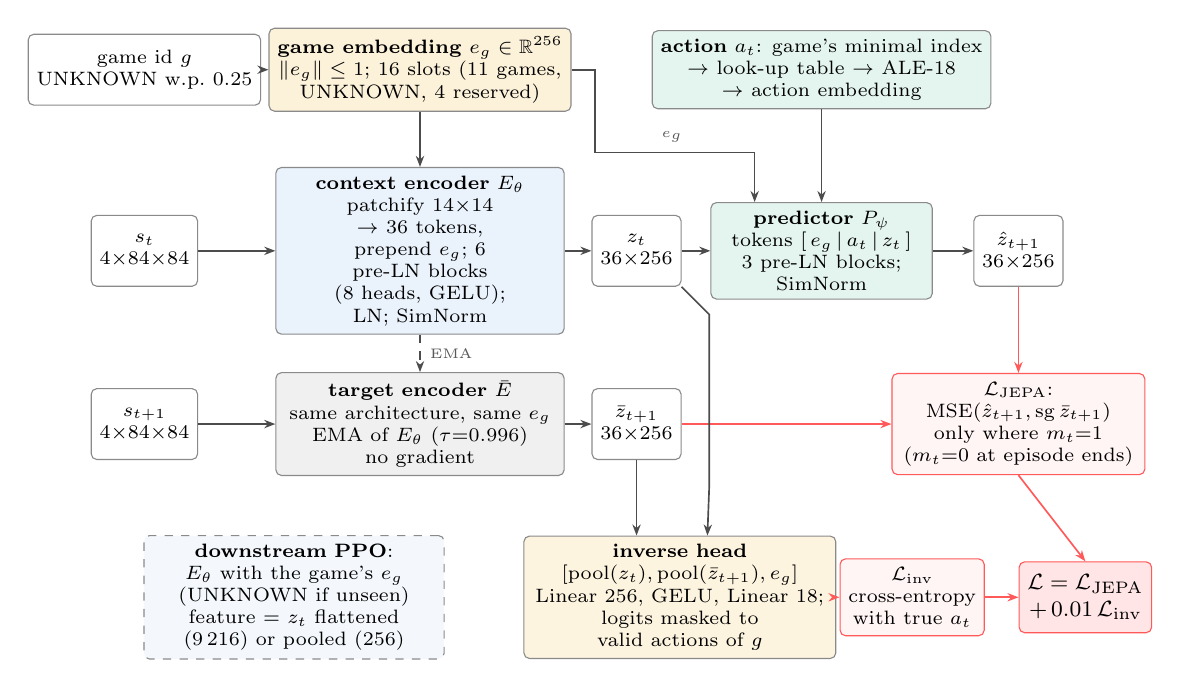
\begin{tikzpicture}[
  font=\scriptsize,
  box/.style={draw=cGray, rounded corners=2pt, align=center, inner sep=3pt, fill=white,
              minimum height=0.9cm},
  arr/.style={-{Stealth[length=4pt]}, draw=black!70, line width=0.6pt},
  larr/.style={-{Stealth[length=4pt]}, draw=red!65, line width=0.6pt},
  lab/.style={font=\tiny, text=black!65}]

  % ---------------------------------------------------------------- conditioning (top row)
  \node[box] (drop) at (0,4.5) {game id $g$\\UNKNOWN w.p.\ 0.25};
  \node[box, fill=cJep!15] (env) at (3.5,4.5)
    {\textbf{game embedding} $e_g\in\mathbb{R}^{256}$\\$\|e_g\|\le1$; 16 slots (11 games,\\UNKNOWN, 4 reserved)};
  \node[box, fill=cFsqJ!12] (act) at (8.6,4.5)
    {\textbf{action} $a_t$: game's minimal index\\$\to$ look-up table $\to$ ALE-18\\$\to$ action embedding};
  \draw[arr] (drop) -- (env);

  % ---------------------------------------------------------------- online branch
  \node[box] (st) at (0,2.2) {$s_t$\\$4{\times}84{\times}84$};
  \node[box, fill=cNat!10, text width=3.45cm] (ce) at (3.5,2.2)
    {\textbf{context encoder} $E_\theta$\\patchify $14{\times}14$ $\to$ 36 tokens,\\prepend $e_g$; 6 pre-LN blocks\\(8 heads, GELU); LN; SimNorm};
  \node[box] (zt) at (6.25,2.2) {$z_t$\\$36{\times}256$};
  \node[box, fill=cFsqJ!12, text width=2.6cm] (pr) at (8.6,2.2)
    {\textbf{predictor} $P_\psi$\\tokens $[\,e_g\,|\,a_t\,|\,z_t\,]$\\3 pre-LN blocks; SimNorm};
  \node[box] (zh) at (11.1,2.2) {$\hat z_{t+1}$\\$36{\times}256$};
  \draw[arr] (st) -- (ce); \draw[arr] (ce) -- (zt); \draw[arr] (zt) -- (pr); \draw[arr] (pr) -- (zh);
  \draw[arr] (env) -- (ce);
  \draw[arr] (act) -- (pr);
  \coordinate (ebend) at (7.75,3.45);
  \draw[arr] (env.east) -- ++(0.3,0) |- (ebend) -- (ebend |- pr.north);
  \node[lab, above] at (6.7,3.45) {$e_g$};

  % ---------------------------------------------------------------- target branch
  \node[box] (sn) at (0,0) {$s_{t+1}$\\$4{\times}84{\times}84$};
  \node[box, fill=gray!12, text width=3.45cm] (te) at (3.5,0)
    {\textbf{target encoder} $\bar E$\\same architecture, same $e_g$\\EMA of $E_\theta$ ($\tau{=}0.996$)\\no gradient};
  \node[box] (zb) at (6.25,0) {$\bar z_{t+1}$\\$36{\times}256$};
  \draw[arr] (sn) -- (te); \draw[arr] (te) -- (zb);
  \draw[arr, dashed] (ce) -- node[right, lab]{EMA} (te);

  % ---------------------------------------------------------------- losses
  \node[box, draw=red!65, fill=red!4, text width=3.0cm] (lj) at (11.1,0)
    {$\mathcal{L}_{\text{JEPA}}$: MSE$(\hat z_{t+1},\operatorname{sg}\bar z_{t+1})$\\only where $m_t{=}1$\\($m_t{=}0$ at episode ends)};
  \draw[larr] (zh) -- (lj);
  \draw[larr] (zb) -- (lj);

  \node[box, fill=cJep!12, text width=3.75cm] (inv) at (6.8,-2.2)
    {\textbf{inverse head}\\$[\operatorname{pool}(z_t),\operatorname{pool}(\bar z_{t+1}),e_g]$\\Linear 256, GELU, Linear 18;\\logits masked to valid actions of $g$};
  \draw[arr] (zt.south east) -- ++(0.35,-0.35) -- ++(0,-2.2) -- ([xshift=0.35cm]inv.north);
  \draw[arr] (zb) -- (zb |- inv.north);
  \node[box, draw=red!65, fill=red!4] (li) at (9.75,-2.2) {$\mathcal{L}_{\text{inv}}$\\cross-entropy\\with true $a_t$};
  \draw[larr] (inv) -- (li);
  \node[box, draw=red!65, fill=red!10, font=\footnotesize] (tot) at (11.95,-2.2)
    {$\mathcal{L}=\mathcal{L}_{\text{JEPA}}$\\$+\,0.01\,\mathcal{L}_{\text{inv}}$};
  \draw[larr] (li) -- (tot);
  \draw[larr] (lj.south) -- (tot.north);

  % ---------------------------------------------------------------- use in PPO
  \node[box, dashed, fill=cNat!5, text width=3.6cm] (ppo) at (1.9,-2.2)
    {\textbf{downstream PPO}: $E_\theta$ with the game's $e_g$ (UNKNOWN if unseen)\\feature = $z_t$ flattened (9\,216) or pooled (256)};
\end{tikzpicture}}

\resizebox{\textwidth}{!}{%
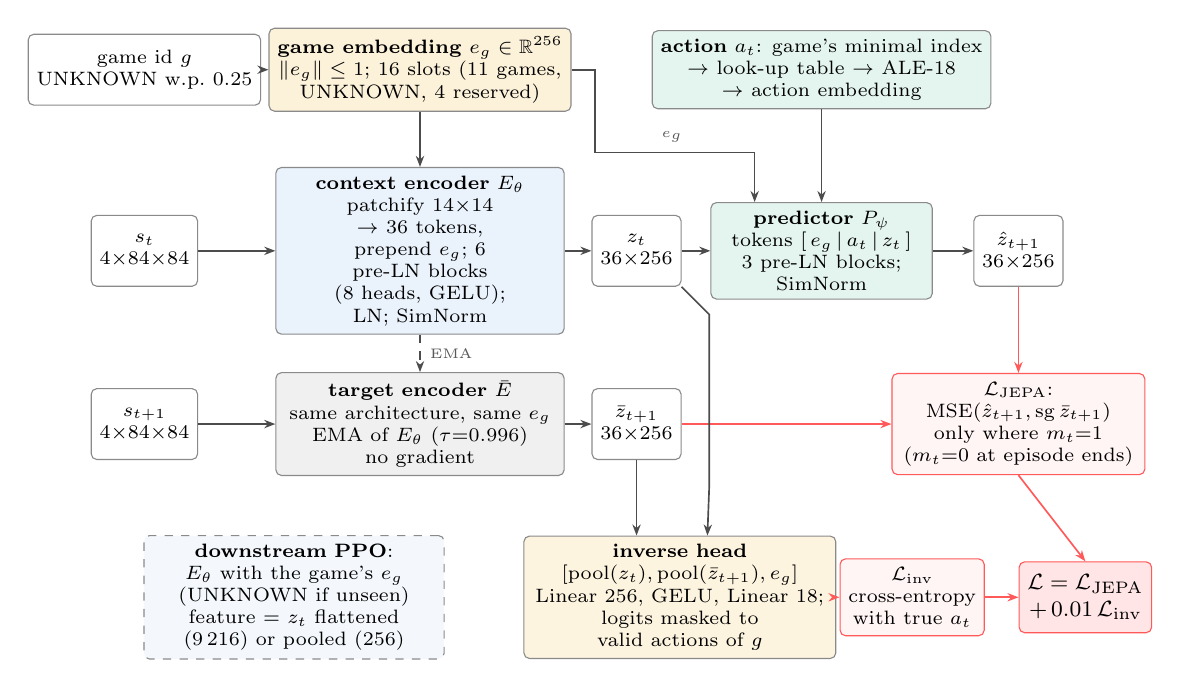
\begin{tikzpicture}[
  font=\scriptsize,
  box/.style={draw=cGray, rounded corners=2pt, align=center, inner sep=3pt, fill=white,
              minimum height=0.9cm},
  arr/.style={-{Stealth[length=4pt]}, draw=black!70, line width=0.6pt},
  larr/.style={-{Stealth[length=4pt]}, draw=red!65, line width=0.6pt},
  lab/.style={font=\tiny, text=black!65}]

  % ---------------------------------------------------------------- conditioning (top row)
  \node[box] (drop) at (0,4.5) {game id $g$\\UNKNOWN w.p.\ 0.25};
  \node[box, fill=cJep!15] (env) at (3.5,4.5)
    {\textbf{game embedding} $e_g\in\mathbb{R}^{256}$\\$\|e_g\|\le1$; 16 slots (11 games,\\UNKNOWN, 4 reserved)};
  \node[box, fill=cFsqJ!12] (act) at (8.6,4.5)
    {\textbf{action} $a_t$: game's minimal index\\$\to$ look-up table $\to$ ALE-18\\$\to$ action embedding};
  \draw[arr] (drop) -- (env);

  % ---------------------------------------------------------------- online branch
  \node[box] (st) at (0,2.2) {$s_t$\\$4{\times}84{\times}84$};
  \node[box, fill=cNat!10, text width=3.45cm] (ce) at (3.5,2.2)
    {\textbf{context encoder} $E_\theta$\\patchify $14{\times}14$ $\to$ 36 tokens,\\prepend $e_g$; 6 pre-LN blocks\\(8 heads, GELU); LN; SimNorm};
  \node[box] (zt) at (6.25,2.2) {$z_t$\\$36{\times}256$};
  \node[box, fill=cFsqJ!12, text width=2.6cm] (pr) at (8.6,2.2)
    {\textbf{predictor} $P_\psi$\\tokens $[\,e_g\,|\,a_t\,|\,z_t\,]$\\3 pre-LN blocks; SimNorm};
  \node[box] (zh) at (11.1,2.2) {$\hat z_{t+1}$\\$36{\times}256$};
  \draw[arr] (st) -- (ce); \draw[arr] (ce) -- (zt); \draw[arr] (zt) -- (pr); \draw[arr] (pr) -- (zh);
  \draw[arr] (env) -- (ce);
  \draw[arr] (act) -- (pr);
  \coordinate (ebend) at (7.75,3.45);
  \draw[arr] (env.east) -- ++(0.3,0) |- (ebend) -- (ebend |- pr.north);
  \node[lab, above] at (6.7,3.45) {$e_g$};

  % ---------------------------------------------------------------- target branch
  \node[box] (sn) at (0,0) {$s_{t+1}$\\$4{\times}84{\times}84$};
  \node[box, fill=gray!12, text width=3.45cm] (te) at (3.5,0)
    {\textbf{target encoder} $\bar E$\\same architecture, same $e_g$\\EMA of $E_\theta$ ($\tau{=}0.996$)\\no gradient};
  \node[box] (zb) at (6.25,0) {$\bar z_{t+1}$\\$36{\times}256$};
  \draw[arr] (sn) -- (te); \draw[arr] (te) -- (zb);
  \draw[arr, dashed] (ce) -- node[right, lab]{EMA} (te);

  % ---------------------------------------------------------------- losses
  \node[box, draw=red!65, fill=red!4, text width=3.0cm] (lj) at (11.1,0)
    {$\mathcal{L}_{\text{JEPA}}$: MSE$(\hat z_{t+1},\operatorname{sg}\bar z_{t+1})$\\only where $m_t{=}1$\\($m_t{=}0$ at episode ends)};
  \draw[larr] (zh) -- (lj);
  \draw[larr] (zb) -- (lj);

  \node[box, fill=cJep!12, text width=3.75cm] (inv) at (6.8,-2.2)
    {\textbf{inverse head}\\$[\operatorname{pool}(z_t),\operatorname{pool}(\bar z_{t+1}),e_g]$\\Linear 256, GELU, Linear 18;\\logits masked to valid actions of $g$};
  \draw[arr] (zt.south east) -- ++(0.35,-0.35) -- ++(0,-2.2) -- ([xshift=0.35cm]inv.north);
  \draw[arr] (zb) -- (zb |- inv.north);
  \node[box, draw=red!65, fill=red!4] (li) at (9.75,-2.2) {$\mathcal{L}_{\text{inv}}$\\cross-entropy\\with true $a_t$};
  \draw[larr] (inv) -- (li);
  \node[box, draw=red!65, fill=red!10, font=\footnotesize] (tot) at (11.95,-2.2)
    {$\mathcal{L}=\mathcal{L}_{\text{JEPA}}$\\$+\,0.01\,\mathcal{L}_{\text{inv}}$};
  \draw[larr] (li) -- (tot);
  \draw[larr] (lj.south) -- (tot.north);

  % ---------------------------------------------------------------- use in PPO
  \node[box, dashed, fill=cNat!5, text width=3.6cm] (ppo) at (1.9,-2.2)
    {\textbf{downstream PPO}: $E_\theta$ with the game's $e_g$ (UNKNOWN if unseen)\\feature = $z_t$ flattened (9\,216) or pooled (256)};
\end{tikzpicture}}
}\\[0.4em]
  {\footnotesize The model predicts the \emph{latent} of the next frame stack, not its pixels.
  The target encoder is a slowly updated copy of the context encoder (no gradients).
  Only the context encoder is used for PPO.\par}
\end{frame}

\begin{frame}{V-JEPA: Design Choices}
  \begin{itemize}\setlength\itemsep{0.3em}
    \item Following TD-MPC2, so that one model can be trained on many games:
      \begin{itemize}\small
        \item one common set of 18 actions (the same index is a different button in each game)
        \item a learnable embedding per game (``UNKNOWN'' 25\% of the time)
        \item SimNorm: latents in groups of 8 with a softmax, against collapse
        \item a head that guesses the action: $\mathcal{L}=\mathcal{L}_{\text{JEPA}}+0.01\,\mathcal{L}_{\text{inv}}$
      \end{itemize}
  \end{itemize}
  \vspace{0.3em}
  \centering
  {\footnotesize
  \begin{tabular}{@{}lrcc@{}}
    \toprule
    Part & Params & learns from $\mathcal{L}_{\text{JEPA}}$ & from $\mathcal{L}_{\text{inv}}$ \\
    \midrule
    Context encoder & 4.95\,M & yes & yes \\
    Predictor & 2.37\,M & yes & no \\
    Inverse head & 0.20\,M & no & yes \\
    Target encoder & 4.95\,M & \multicolumn{2}{c}{moving average only} \\
    \bottomrule
  \end{tabular}}
\end{frame}

\begin{frame}{Experimental Setup: Pre-Training}
  \centering
  {\scriptsize\setlength{\tabcolsep}{3pt}
  \begin{tabular}{@{}lcccc@{}}
    \toprule
    & Std.\ VAE & Res.\ VQ-VAE & FSQ-VAE & V-JEPA \\
    \midrule
    Data & 550\,k stacks & 550\,k stacks & 550\,k stacks & 2.75\,M transitions \\
    Length & 58 epochs & 29 epochs & 125 epochs & 92 epochs \\
    Steps & 250\,k & 250\,k & 537\,k & 494\,k \\
    Batch & 128 & 64 & 128 & 512 \\
    Optimiser, LR & Adam, $10^{-3}$ & $3{\cdot}10^{-4}$ & AdamW, $3{\cdot}10^{-4}$ & AdamW, $3{\cdot}10^{-4}$ \\
    Parameters & 2.56\,M & 0.70\,M & 0.84\,M & 12.5\,M \\
    Hardware, time & H100, 0.8\,h & H100, 0.9\,h & H100, 1.9\,h & H100, 15.6\,h \\
    \bottomrule
  \end{tabular}}
  \vspace{0.8em}
  \begin{itemize}\small\setlength\itemsep{0.4em}
    \item The architectures follow the original papers (VQ-VAE, FSQ, I-JEPA, TD-MPC2)
    \item The JEPA papers train huge models on many GPUs, so a smaller batch (512) and a lower
          learning rate were used for the 12.5\,M model on one GPU
    \item For the V-JEPA, the checkpoint with the lowest total validation loss
          $\mathcal{L}_{\text{JEPA}}+0.01\,\mathcal{L}_{\text{inv}}$ (epoch 92) was used; a small
          sweep confirmed the inverse-loss weight $\lambda=0.01$
  \end{itemize}
\end{frame}

\begin{frame}{Experimental Setup: PPO and Evaluation}
  \begin{itemize}\setlength\itemsep{0.55em}
    \item \textbf{Baseline:} NatureCNN trained from scratch
    \item \textbf{Frozen:} pre-trained encoder stays fixed, only the actor and critic learn
    \item \textbf{Fine-tuned:} pre-trained encoder keeps learning together with the policy
    \item \textbf{PPO:} standard RL-Zoo Atari settings, 10\,M steps, same 512-unit heads for
          every encoder
    \item \textbf{Metric:} mean return over the last 1\,M steps, turned into the
          human-normalised score so that games can be compared
      \[\text{HNS}=\frac{\text{score}-\text{random}}{\text{human}-\text{random}}\]
    \item One seed per run; all numbers come from the full Weights \& Biases logs
  \end{itemize}
\end{frame}

\begin{frame}{Scope of the Work}
  \centering
  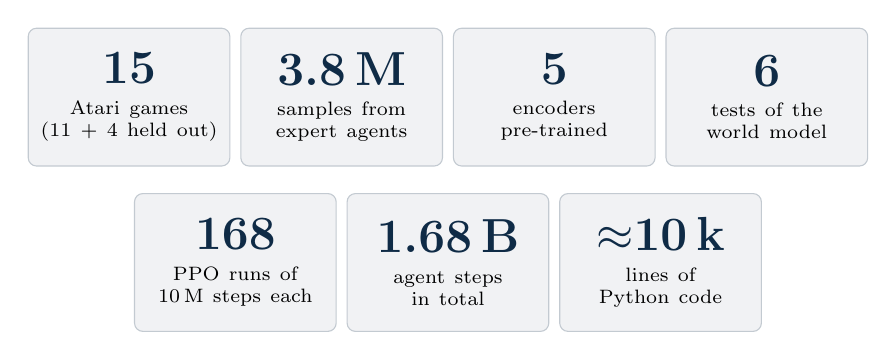
\begin{tikzpicture}[
    tile/.style={rounded corners=3pt, fill=tudnavy!6, draw=tudnavy!25, align=center,
                 text width=2.35cm, minimum height=1.75cm, inner sep=3pt}]
    \stat{0,0}{15}{Atari games\\(11 + 4 held out)}
    \stat{2.7,0}{3.8\,M}{samples from\\expert agents}
    \stat{5.4,0}{5}{encoders\\pre-trained}
    \stat{8.1,0}{6}{tests of the\\world model}
    \stat{1.35,-2.1}{168}{PPO runs of\\10\,M steps each}
    \stat{4.05,-2.1}{1.68\,B}{agent steps\\in total}
    \stat{6.75,-2.1}{$\approx$10\,k}{lines of\\Python code}
  \end{tikzpicture}\\[1.2em]
  {\footnotesize PPO runs: NatureCNN 15 $\cdot$ Std-VAE 30 $\cdot$ Res-VQ 30 $\cdot$ FSQ-VAE 30 $\cdot$
  V-JEPA 63}\\[0.2em]
  {\footnotesize May--September 2026, ZIH \emph{Capella} cluster (NVIDIA H100)}
\end{frame}

% =================================================================
\section{Results}

\begin{frame}{Pre-Training Results}
  \centering
  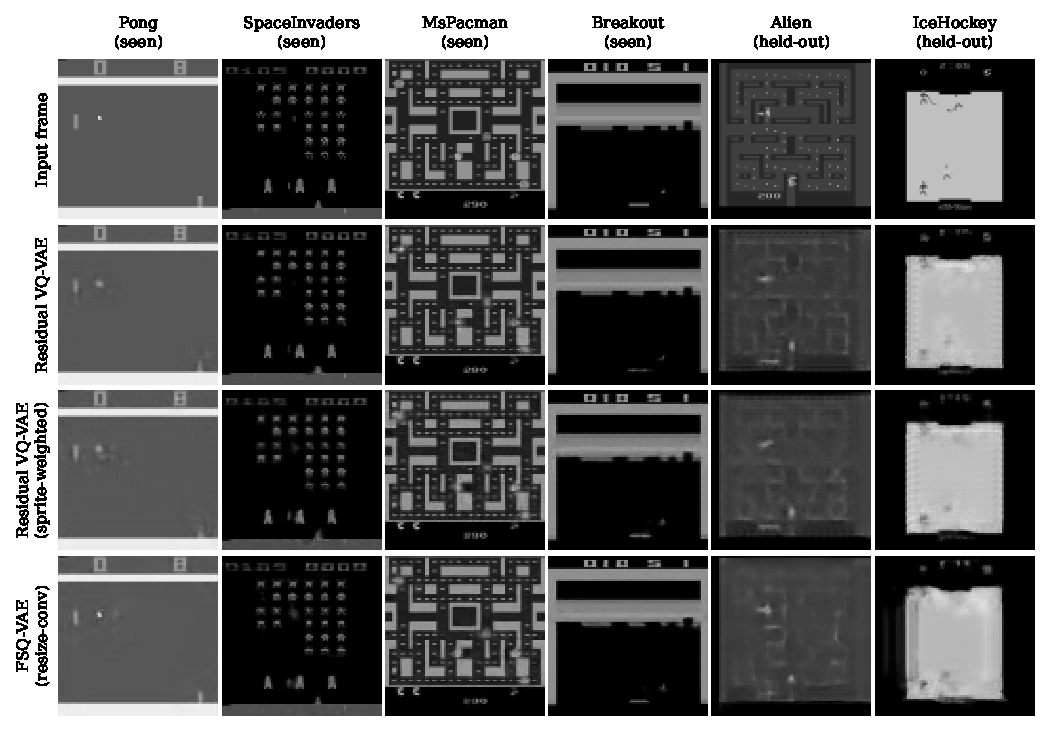
\includegraphics[width=0.74\textwidth]{figures/reconstructions.pdf}
  \begin{itemize}\footnotesize\setlength\itemsep{0.1em}
    \item \textbf{FSQ-VAE:} lowest error, and $3\times$ less error on moving pixels than the VQ-VAE
    \item \textbf{Held-out games:} all autoencoders are much worse; they fit the training games
    \item \textbf{V-JEPA:} the loss went \emph{up} after epoch 2 while the latents became richer
          (effective rank $1.4\to57$); the low early loss came from almost collapsed latents
  \end{itemize}
\end{frame}

\begin{frame}{Downstream RL Performance}
  \centering
  {\footnotesize\setlength{\tabcolsep}{2.5pt}
  \resizebox{0.9\textwidth}{!}{%
  \begin{tabular}{@{}lcccccccccc@{}}
    \toprule
    & NatureCNN & \multicolumn{2}{c}{Std-VAE} & \multicolumn{2}{c}{Res-VQ} & \multicolumn{2}{c}{FSQ-VAE} & \multicolumn{2}{c}{V-JEPA} \\
    \cmidrule(lr){3-4}\cmidrule(lr){5-6}\cmidrule(lr){7-8}\cmidrule(lr){9-10}
    & scratch & frzn & joint & frzn & joint & frzn & joint & frzn & joint \\
    \midrule
    Med HNS (seen) & 0.74 & 0.06 & 0.36 & 0.17 & 0.85 & 0.31 & \textbf{1.07} & 0.05 & 0.04 \\
    Mean HNS (seen) & \textbf{2.51} & 0.14 & 0.53 & 0.30 & 0.91 & 0.54 & 2.02 & 0.13 & 0.07 \\
    Med HNS (held-out) & \textbf{0.50} & 0.01 & 0.05 & 0.05 & 0.21 & 0.21 & 0.45 & 0.05 & 0.06 \\
    \bottomrule
  \end{tabular}}}\\[0.2em]
  {\tiny Std-VAE, Res-VQ and the NatureCNN/V-JEPA held-out scores were recorded rounded}
  \vspace{0.2em}
  \begin{itemize}\small\setlength\itemsep{0.12em}
    \item \textbf{FSQ fine-tuned:} highest median (1.07 vs.\ 0.74), beat NatureCNN on 4 of 11
          games and nearly tied on Pong and Seaquest
    \item NatureCNN stayed ahead on the other games (about $2\times$ on DemonAttack and
          RoadRunner), so its mean is higher
    \item \textbf{Other VAEs:} Std-VAE lowest on every game; Res-VQ below FSQ except on MsPacman,
          furthest behind on small, fast sprites
    \item \textbf{FSQ frozen:} learned something in every game, but reached less than a third
          of the fine-tuned median
    \item \textbf{FSQ:} fine-tuning beat freezing on 13 of 15 games (Breakout $12\times$)
    \item \textbf{Held-out games:} NatureCNN ahead of FSQ fine-tuned on 3 of 4
    \item \textbf{V-JEPA:} learned very little, frozen or fine-tuned
  \end{itemize}
\end{frame}

\begin{frame}{Learning Curves}
  \centering
  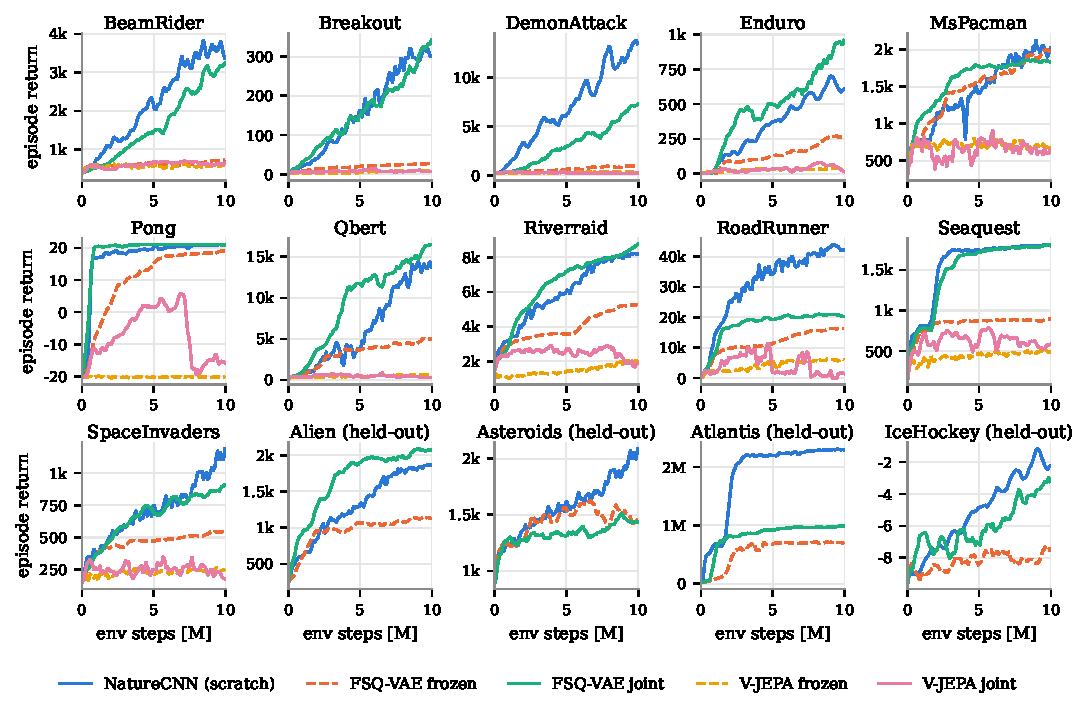
\includegraphics[width=\textwidth]{figures/learning_curves.pdf}\\[0.2em]
  {\footnotesize Solid: trained or fine-tuned encoders; dashed: frozen encoders}
\end{frame}

\begin{frame}{Sample Efficiency}
  \centering
  {\scriptsize Million steps until an agent first covers 50\% / 80\% of NatureCNN's learning
  progress (--: never); fastest in bold\par}\vspace{0.3em}
  {\scriptsize\setlength{\tabcolsep}{6pt}\renewcommand{\arraystretch}{1.05}
  \begin{tabular}{@{}lcccccc@{}}
    \toprule
     & \multicolumn{3}{c}{50\% level} & \multicolumn{3}{c}{80\% level} \\
    \cmidrule(lr){2-4}\cmidrule(lr){5-7}
    Game & Nature & FSQ-J & FSQ-F & Nature & FSQ-J & FSQ-F \\
    \midrule
    \tabinput{tables/sample_eff_rows.tex}
    \bottomrule
  \end{tabular}}\\[0.3em]
  \begin{itemize}\footnotesize\setlength\itemsep{0.1em}
    \item FSQ fine-tuned (FSQ-J) reached the 80\% level 1.4--2.6\,M steps earlier on Enduro,
          MsPacman, Qbert and Riverraid
    \item FSQ frozen (FSQ-F) reached the 80\% level on only 2 of 11 games
  \end{itemize}
\end{frame}

\begin{frame}{V-JEPA: Can the Features Be Fixed?}
  \begin{itemize}\setlength\itemsep{0.55em}
    \item Hypothesis: the 9\,216-dimensional feature is too big for PPO
    \item All 22 seen-game runs were repeated with the tokens averaged into a \textbf{256-dim}
          feature (these runs also used separate actor and critic encoders)
    \item The frozen runs were repeated with a $5\times$ larger \textbf{entropy bonus}
  \end{itemize}
  \vspace{0.3em}
  \centering
  {\small
  \begin{tabular}{@{}llcc@{}}
    \toprule
    Feature & Mode & Median HNS & Critic expl.\ var. \\
    \midrule
    9\,216 (flat) & frozen & 0.045 & 0.73 \\
    256 (pooled) & frozen & 0.021 & 0.53 \\
    256 (pooled) & fine-tuned & 0.007 & $-0.27$ \\
    256, entropy 0.05 & frozen & 0.015 & 0.03 \\
    \bottomrule
  \end{tabular}}
  \vspace{0.5em}
  \begin{itemize}\small
    \item Neither change helped, so the size of the feature was probably not the problem, but
          the information in it
  \end{itemize}
\end{frame}

\begin{frame}{V-JEPA: World-Model Diagnostics}
  \begin{columns}[T]
    \begin{column}{0.57\textwidth}
      \begin{itemize}\small\setlength\itemsep{0.2em}
        \item Next states share 3 of 4 frames, so \textbf{copying} the current latent already
              looks good. Baselines: copying, an untrained model and \textbf{wrong actions}
        \item \textbf{No collapse:} effective rank 52.5 vs.\ 2.5 untrained
        \item \textbf{It learned dynamics:} better than copying, gap grows from $+0.013$
              (1 step) to $+0.046$ (5 steps)
        \item \textbf{But the action barely matters:} a wrong action changes the prediction by
              only 0.006
        \item The game token gets $1.8\times$ uniform attention, but the encoder already
              recognises the game from the pixels
        \item On held-out games it is worse than copying
      \end{itemize}
    \end{column}
    \begin{column}{0.43\textwidth}
      \centering
      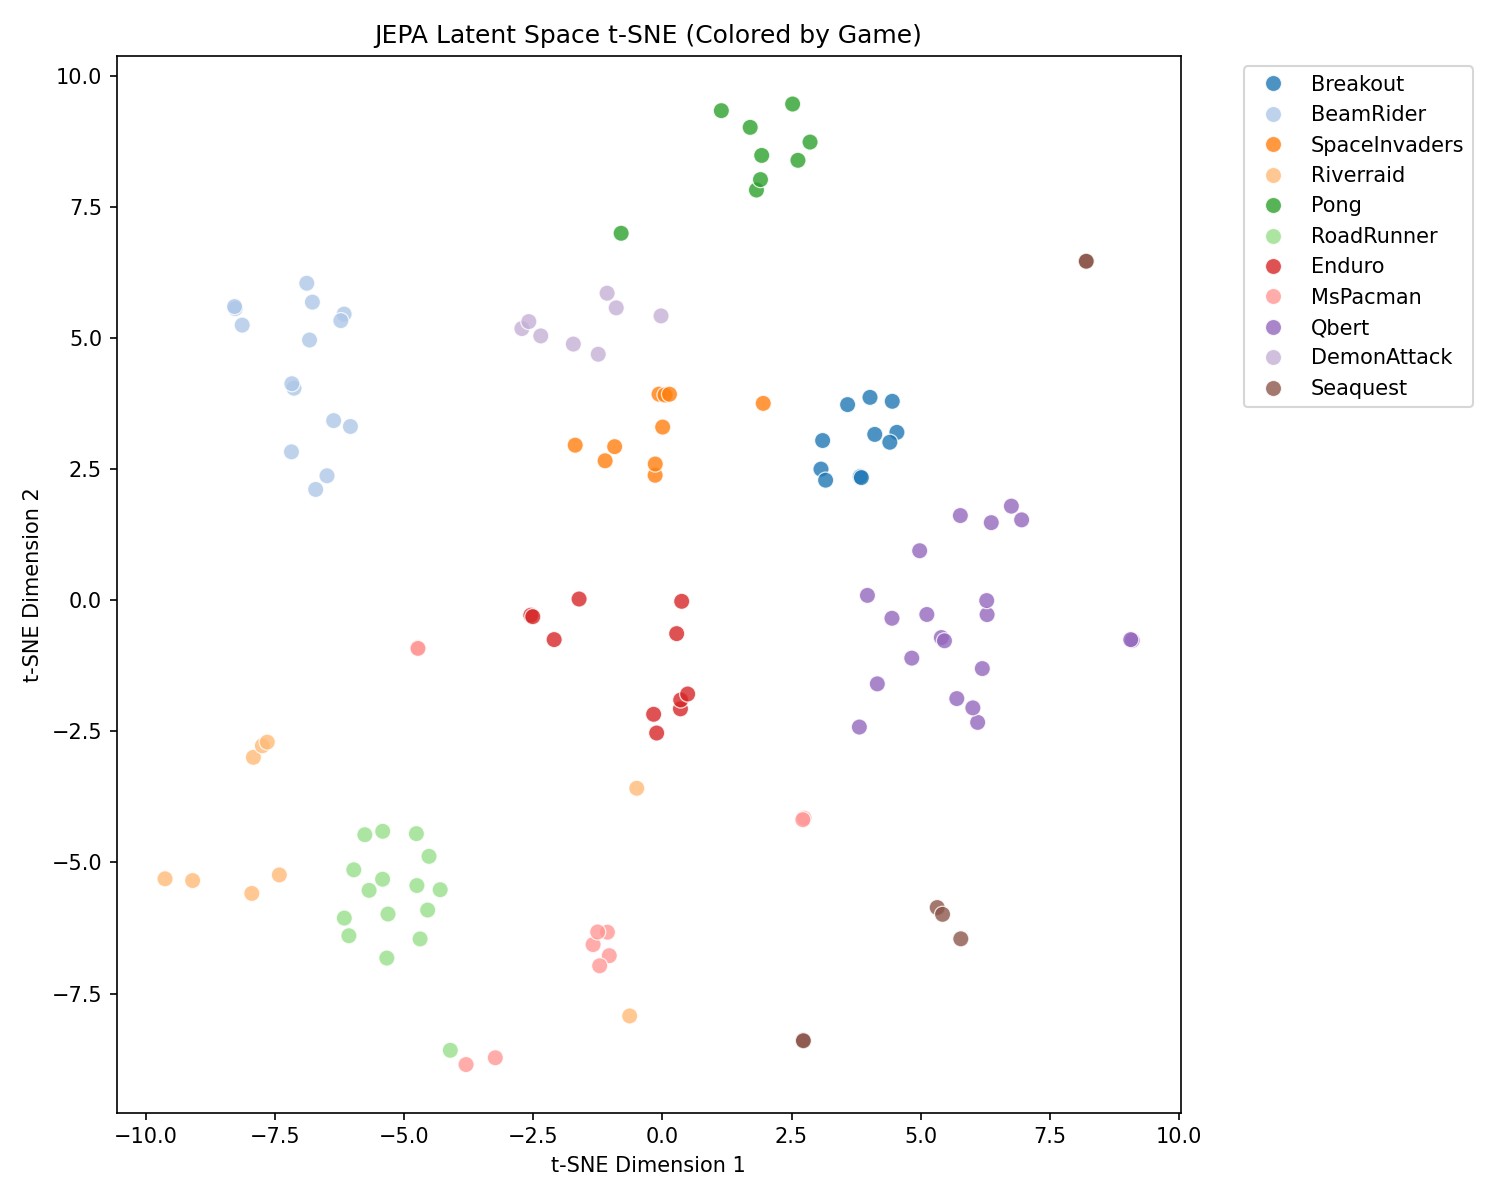
\includegraphics[width=\textwidth]{figures/jepa_tsne_by_game.png}\\[0.2em]
      {\scriptsize t-SNE of V-JEPA latents: they group by game\par}
    \end{column}
  \end{columns}
\end{frame}

\begin{frame}{Why the V-JEPA Fails with PPO}
  \begin{columns}[T]
    \begin{column}{0.46\textwidth}
      \centering
      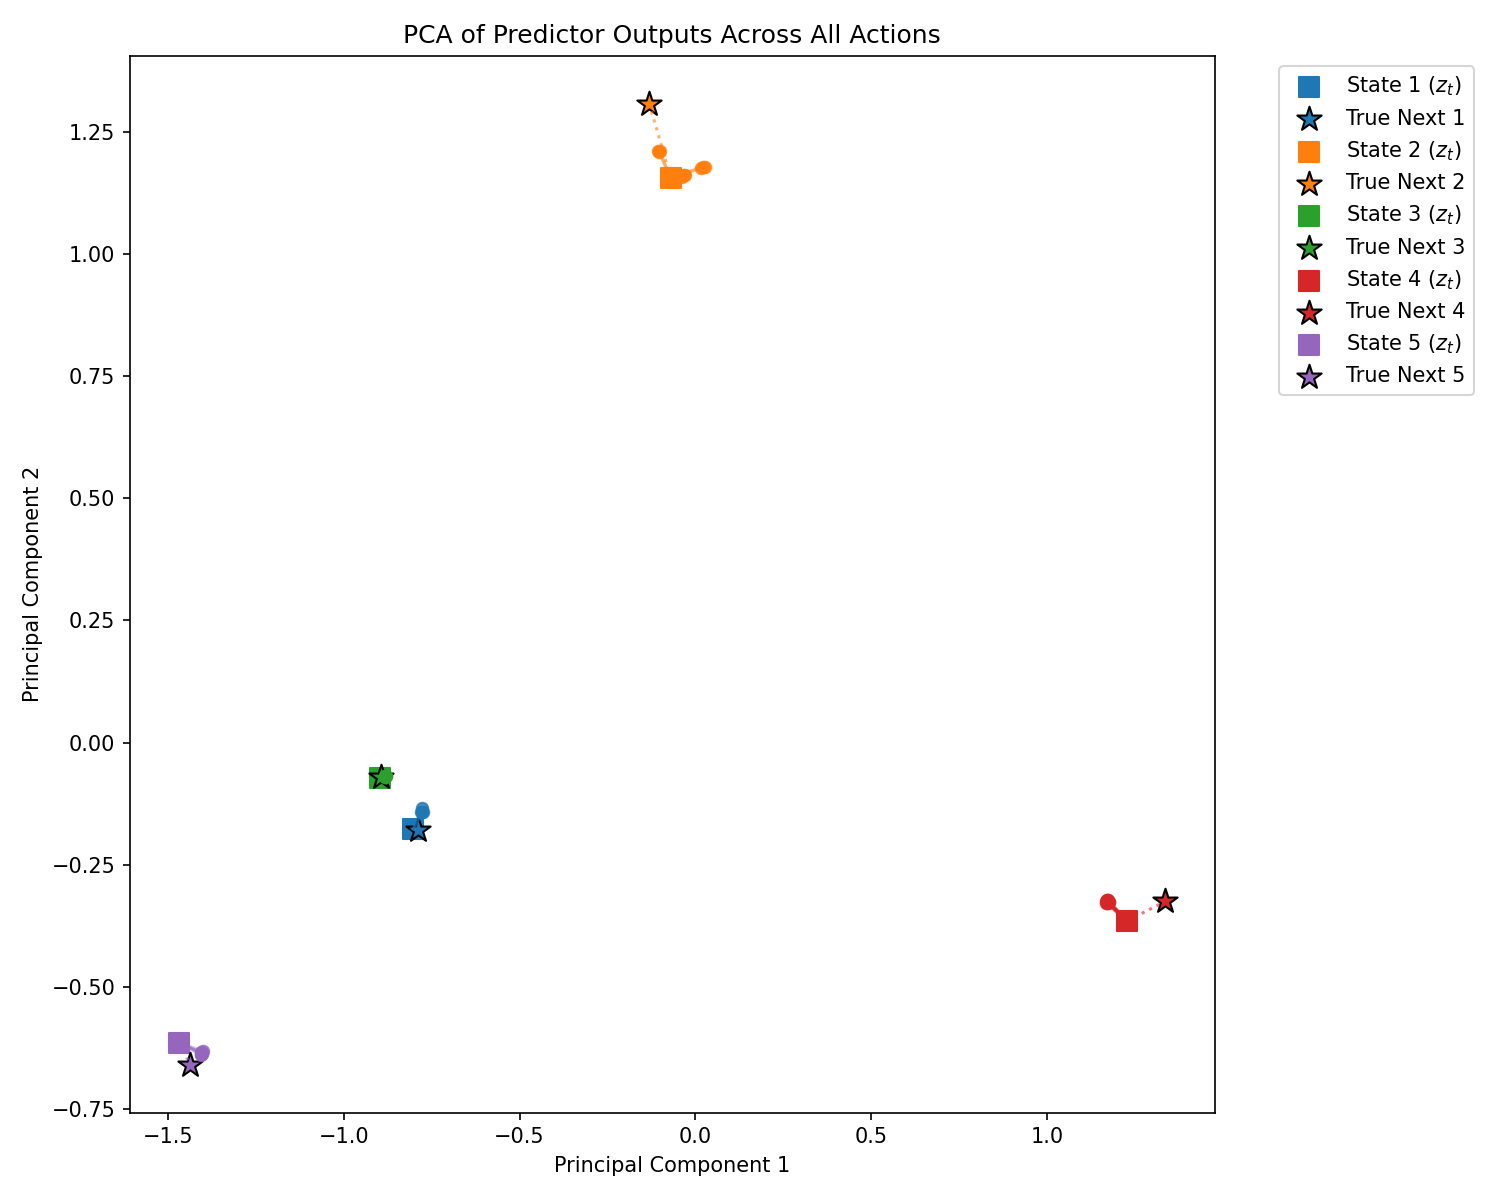
\includegraphics[width=\textwidth]{figures/pca_action_sensitivity.png}\\[0.2em]
      {\scriptsize The predictions for all actions (dots) land almost on the same spot\par}
    \end{column}
    \begin{column}{0.54\textwidth}
      \footnotesize
      \textbf{Observations}
      \begin{itemize}\setlength\itemsep{0.1em}
        \item Predictor mostly ignores the action
        \item Latents barely change per step (cos.\ 0.974)
        \item Latent space is sorted by game
        \item Worse on held-out games
      \end{itemize}
      \vspace{0.3em}
      \textbf{Interpretation}
      \begin{itemize}\setlength\itemsep{0.1em}
        \item JEPA can ignore details with little effect on the latent error, like a small
              ball
        \item $14\times14$ patches are coarse for small objects
        \item Expert data shows few other actions
        \item The critic could read how good a state is, but the policy could not find the
              right action
      \end{itemize}
    \end{column}
  \end{columns}
\end{frame}

\begin{frame}{Compute Cost and Energy}
  \centering
  {\footnotesize\setlength{\tabcolsep}{4pt}
  \begin{tabular}{@{}llrcc@{}}
    \toprule
    & & & \multicolumn{2}{c}{per run} \\
    \cmidrule(lr){4-5}
    Stage & Model & Runs & GPU-h & kWh \\
    \midrule
    Pre-training & Std-VAE / Res-VQ$^{*}$ & 3 & 0.8 / 0.9 & 0.29 / 0.33 \\
     & FSQ-VAE & 1 & 1.9 & 0.70 \\
     & V-JEPA & 1 & 15.6 & 1.96 \\
    \midrule
    PPO (10\,M steps) & NatureCNN & 15 & 3.1 & 0.39 \\
     & Std-VAE, Res-VQ$^{*}$ & 60 & 2.2 & 0.32 \\
     & FSQ-VAE & 30 & 2.2 & 0.31 \\
     & V-JEPA frozen / fine-tuned & 30 & 3.6 / 4.5 & 0.55 / 0.84 \\
     & V-JEPA ablations & 33 & 4.0 & 0.67 \\
    \midrule
    \textbf{Total} & reported experiments & 177 & \multicolumn{2}{c}{\textbf{$\approx$520 GPU-h, 82 kWh}} \\
    \bottomrule
  \end{tabular}}\\[0.2em]
  {\tiny per run: mean over runs; $^{*}$\,approximate (not logged in W\&B); energy = measured GPU power, one NVIDIA H100 per run}
  \vspace{0.3em}
  \begin{itemize}\footnotesize\setlength\itemsep{0.15em}
    \item Pre-training is a \textbf{one-off cost} of about one PPO run and is shared by all games
    \item During PPO the GPU is mostly idle (the Atari emulator runs on the CPU): 125--210\,W of 700\,W
    \item \textbf{Interpretability:} the autoencoder decoders turn features back into images; the
          V-JEPA can only be inspected indirectly (PCA, t-SNE, probes)
  \end{itemize}
\end{frame}

% =================================================================
\section{Conclusion}

\begin{frame}{Conclusion}
  \begin{itemize}\small\setlength\itemsep{0.35em}
    \item \textbf{RQ1:} the FSQ-VAE gave the most useful features when fine-tuned (beat Std-VAE on every game,
          Res-VQ on all but one)
    \item \textbf{RQ2:} fine-tuning worked much better than freezing
      \begin{itemize}
        \item FSQ fine-tuned vs.\ NatureCNN: higher median HNS (1.07 vs.\ 0.74) and faster
              learning on 4 games, but a better final score on only 4 of 11
      \end{itemize}
    \item \textbf{RQ3:} no overall gain on unseen games (FSQ better only on Alien, NatureCNN
          ahead on the other 3)
    \item \textbf{RQ4:} pre-training costs about one PPO run (FSQ-VAE: 1.9\,GPU-h, 0.7\,kWh) and is
          shared by all games; all experiments took $\approx$520\,GPU-h and 82\,kWh. The FSQ
          decoder shows what the features contain
    \item The V-JEPA learned how games usually evolve, but hardly what the agent's actions change
    \item \textbf{Overall:} a shared encoder is a useful starting point, but it cannot yet
          replace the NatureCNN when frozen
  \end{itemize}
\end{frame}

\begin{frame}{Limitations and Future Work}
  \begin{itemize}\setlength\itemsep{0.55em}
    \item \textbf{Limitations:} one seed per run, PPO not re-tuned for the pre-trained encoders
    \item \textbf{Future work:}
      \begin{itemize}\setlength\itemsep{0.3em}
        \item Repeat the main comparison with 3 seeds
        \item V-JEPA with smaller patches and a loss where the action matters more
              (multi-step prediction, reward head)
        \item Check the features first by predicting object positions, before running PPO
        \item Use the FSQ grid inside a world model, and pre-train on more games
      \end{itemize}
  \end{itemize}
\end{frame}

\begin{frame}
  \vfill
  \centering
  {\Huge\bfseries Thank You!}\\[1em]
  {\Large Questions?}
  \vfill
\end{frame}

\end{document}
